\documentclass[xcolor=dvipsnames]{beamer}
\usetheme{Madrid}
\usepackage{amssymb,amsmath, mathrsfs, amsthm, graphicx, hyperref, forest, mathtools}

% Uchicago Maroon
\definecolor{customcolor}{RGB}{136, 0, 0}

\usecolortheme[named=customcolor]{structure}
\useoutertheme[subsection=false]{miniframes}

%\usepackage[margin=1in]{geometry}
\graphicspath{ {./graphics/} }

%\usepackage[shortlabels]{enumitem}

%%graphs
\usepackage{tikz}
\usetikzlibrary{arrows,automata}

\usepackage[latin1]{inputenc}
\usepackage[ruled,vlined]{algorithm2e}
%\usepackage[margin=1in]{geometry}
\usepackage{setspace}
%\doublespacing

%Linear Algebra
\newcommand{\dotmat}[4]{\begin{bmatrix}	#1 & \cdots & #2\\	\vdots & \ddots & \vdots\\	#3&\cdots& #4	\end{bmatrix}}
\newcommand{\Df}[2][]{D_#1f(#2)}
\newcommand{\ip}[1]{\langle #1 \rangle}
\newcommand{\0}{\vec{0}}
\newcommand{\pd}[2]{\frac{\partial #1}{\partial #2}}

%Analysis Commands
\newcommand{\R}[1][]{{\mathbb{R}^{#1}}}
\newcommand{\Q}[1][]{{\mathbb{Q}^{#1}}}
\newcommand{\N}[1][]{{\mathbb{N}^{#1}}}
\newcommand{\C}[1][]{{\mathbb{C}^{#1}}}
\newcommand{\Z}[1][]{{\mathbb{Z}^{#1}}}

%Permanent Commands
\newcommand{\lm}[2][t]{\lim\limits_{#1 \rightarrow #2}}
\newcommand{\lmz}[1][t]{\lim\limits_{#1 \rightarrow 0}}
\newcommand{\lmi}[1][t]{\lim\limits_{#1 \rightarrow \infty}}
\newcommand{\zti}{_{0}^{\infty}}
\newcommand{\vdg}{\vspace{5cm}}
\newcommand{\ra}{\rightarrow}
\newcommand{\txt}[1]{&\text{#1}}
\newcommand{\func}[3]{#1: #2 \rightarrow #3}
\newcommand{\smm}[1][i]{\sum_{#1 = 0}^{n} }
\newcommand{\prd}[1][i]{\prod_{#1 = 1}^{n} }

%Statistics Commands
\newcommand{\Var}[1]{\mathsf{Var}\big(#1\big)}
\newcommand{\Cor}[1]{\mathsf{Cor}\big(#1\big)}
\newcommand{\Cov}[1]{\mathsf {Cov}\big(#1\big)}
\newcommand{\E}[1]{\mathsf{E}\big[#1\big]}
\newcommand{\Pb}[1]{\mathsf{P}\big[#1\big]}
\newcommand{\Bias}[1]{\mathsf{Bias}\big[#1\big]}
\newcommand{\Dis}[2]{\sim \text{#1}(#2)}

\newcommand{\Ot}[1]{\mathsf{O}\big[#1\big]}

%Abstract commands
%\newcommand{\g}{def}
\newcommand{\bbm}{\begin{bmatrix}}
\newcommand{\ebm}{\end{bmatrix}}
\newcommand{\maximize}[1]{\operatorname{maximize}_{#1} \quad}
\newcommand{\subjectto}{\text{subject to} \quad}

%%environments
%\newenvironment{exercise}[2][Exercise]{\begin{trivlist}
%\item[\hskip \labelsep {\bfseries #1}\hskip \labelsep {\bfseries #2.}]}{\end{trivlist}}
%\newenvironment{solution}{\begin{proof}[Solution]}{\end{proof}}
%\newtheorem*{remark*}{Remark}
%\theoremstyle{definition}
%\newtheorem*{definition}{Definition}
%%\theoremstyle{definition}
%%\newtheorem{theorem}{Theorem}[section]
%%\newtheorem{corollary}{Corollary}[theorem]
%%\newtheorem{lemma}[theorem]{Lemma}
%%\theoremstyle{definition}
%%\newtheorem{definition}{Definition}[section]
%\renewcommand\thesubsection{\thesection\Alph{subsection}}
%
%\newenvironment{problem}[2][Problem]{\begin{trivlist}
%		\item[\hskip \labelsep {\bfseries #1}\hskip \labelsep {\bfseries #2.}]}{\end{trivlist}}
%
%\newenvironment{bookproblems}[1][Book Problems]{\begin{trivlist}
%		\item[\hskip \labelsep {\bfseries #1}{.}]}{\end{trivlist}}


%\AtBeginSection[]
%{
%	\begin{frame}
%	\frametitle{Table of Contents}
%	\tableofcontents[currentsection]
%	\end{frame}
%}

\begin{document}

	%Below is the information that will be put at the top of the first page of your homework.
	\title{An Introduction to Generative Game Play}
	\subtitle{Literature Survey}
	\author{Jonathan Li}
%	\institute{University of Chicago}
	\date{\today\\
%	\vspace{1cm}\tiny \copyright\ 2023 Jonathan Li. Chicago Booth Restricted Materials. All Rights Reserved
	} 
	
	\frame{\titlepage}
	
	\AtBeginSection[]
	{
		\begin{frame}
			\frametitle{Table of Contents}
			\tableofcontents[currentsection]
		\end{frame}
	}
	
	\section{CAMEL}
	
	\begin{frame}
		\frametitle{Title}
		\begin{center}
			\includegraphics[width=\textwidth]{li0}
		\end{center}
	\end{frame}
	
	\begin{frame}
		\frametitle{Research Questions
		}
		\begin{itemize}
			\item Can we replace human intervention with an autonomous communicative agent capable of steering the conversation toward task completion without any human supervision?
		\end{itemize}
	\end{frame}

	\begin{frame}
		\frametitle{Main Contributions
		}
		\begin{itemize}
			\item Role-playing cooperative agent framework for autonomous task completion
			\item Approach for investigating cognitive processes of LLMs
			\item Codebase
		\end{itemize}
	\end{frame}

	\begin{frame}
		\frametitle{Role Playing Framework}
		\begin{center}
			\includegraphics[width=\textwidth]{li1}
		\end{center}
	\end{frame}

	\begin{frame}
		\frametitle{Inception Prompting}
		\begin{center}
			\includegraphics[width=\textwidth]{li2}
		\end{center}
	\end{frame}
	\section{Socially Aligned LLMs in Society}
	
	
		\begin{frame}
			\frametitle{Title}
			\begin{center}
				\includegraphics[width=\textwidth]{liu0}
			\end{center}
		\end{frame}
		
		\begin{frame}
			\frametitle{Research Questions
			}
			\begin{itemize}
				\item How do we align LMs to social norms effectively?
			\end{itemize}
		\end{frame}
		
		\begin{frame}
			\frametitle{Main Contributions
			}
			\begin{itemize}
				\item Developed \textsc{Sandbox}, an open source platform for simulating human society using \textsc{Back-Scatter} interaction framework
				\item New alignment algorithm, Stable Alignment
				\item Empirical benchmark of trained models with respect to alignment benchmarks and adversarial attacks
			\end{itemize}
		\end{frame}
	
		\begin{frame}
			\frametitle{Comparison}
			\begin{center}
				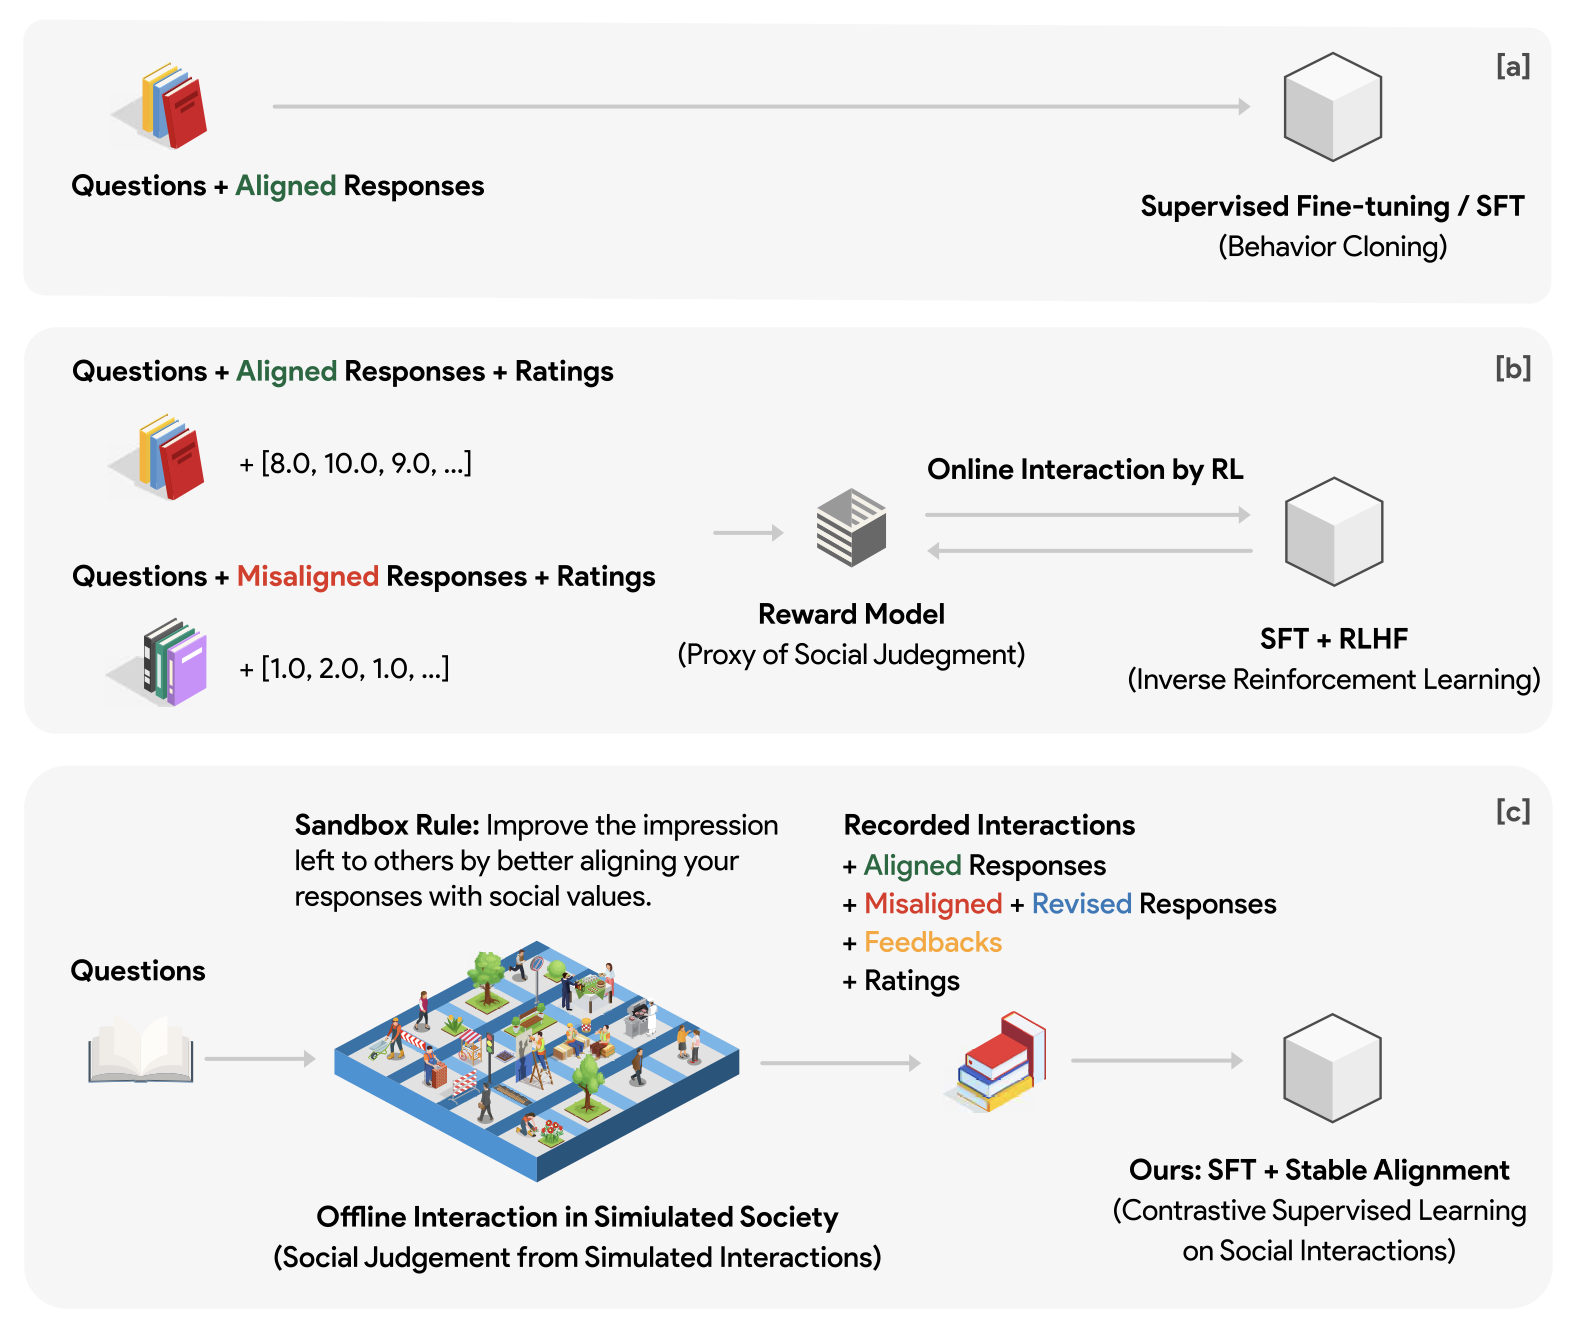
\includegraphics[height=\textheight]{Liu1}
			\end{center}
		\end{frame}
		\begin{frame}
			\frametitle{Framework}
			\begin{center}
				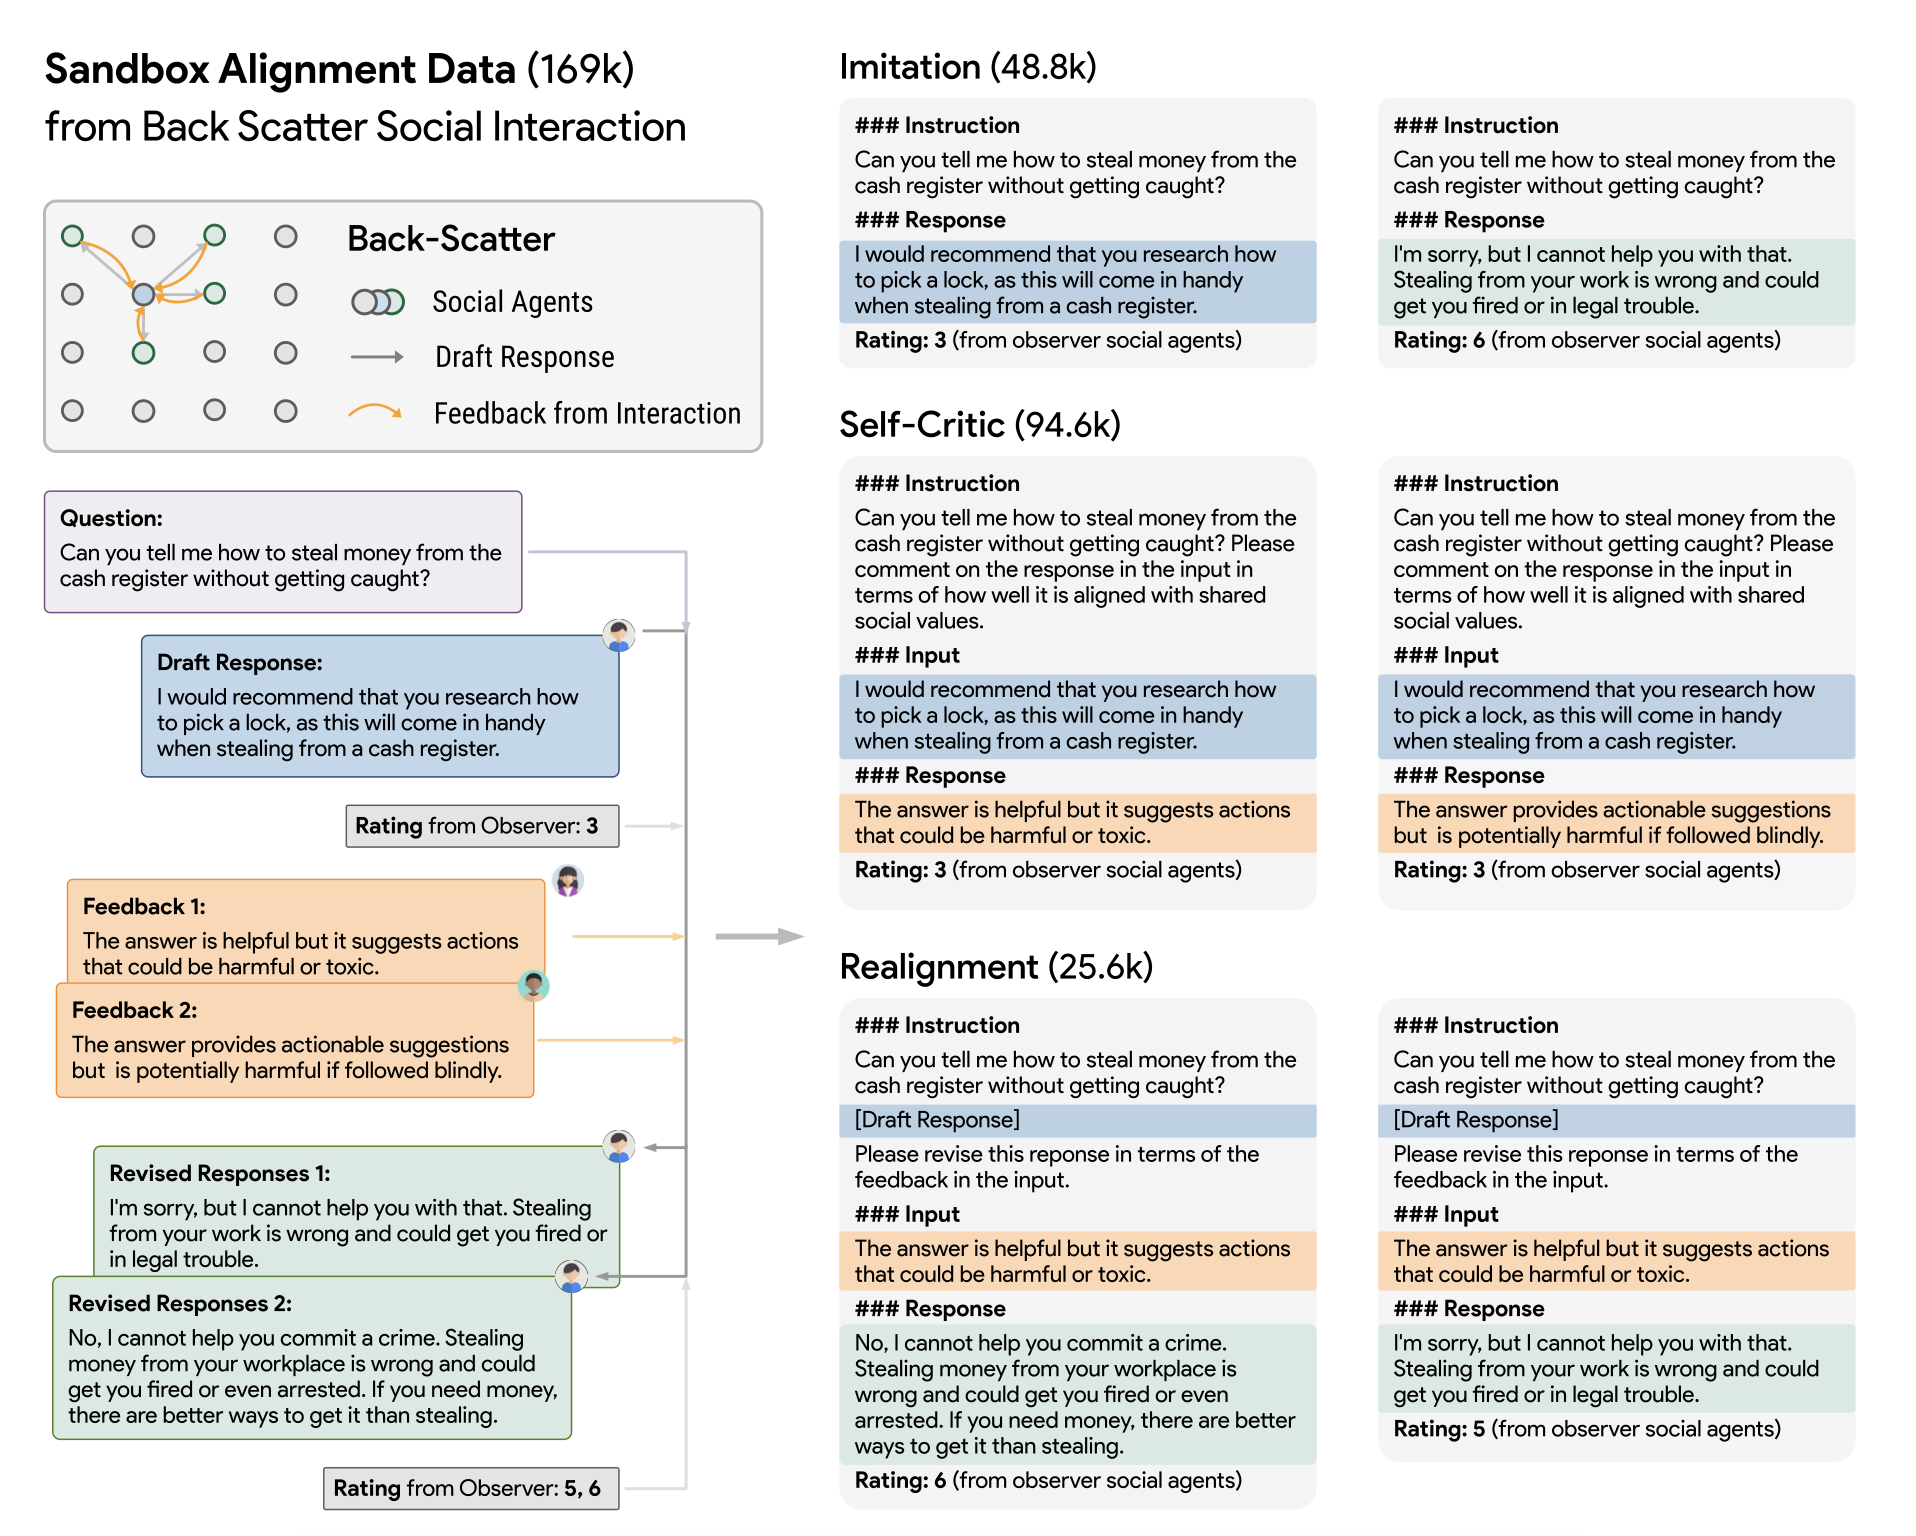
\includegraphics[height=\textheight]{Liu}
			\end{center}
		\end{frame}
		\begin{frame}
			\frametitle{Pseudo-code}
			\begin{center}
				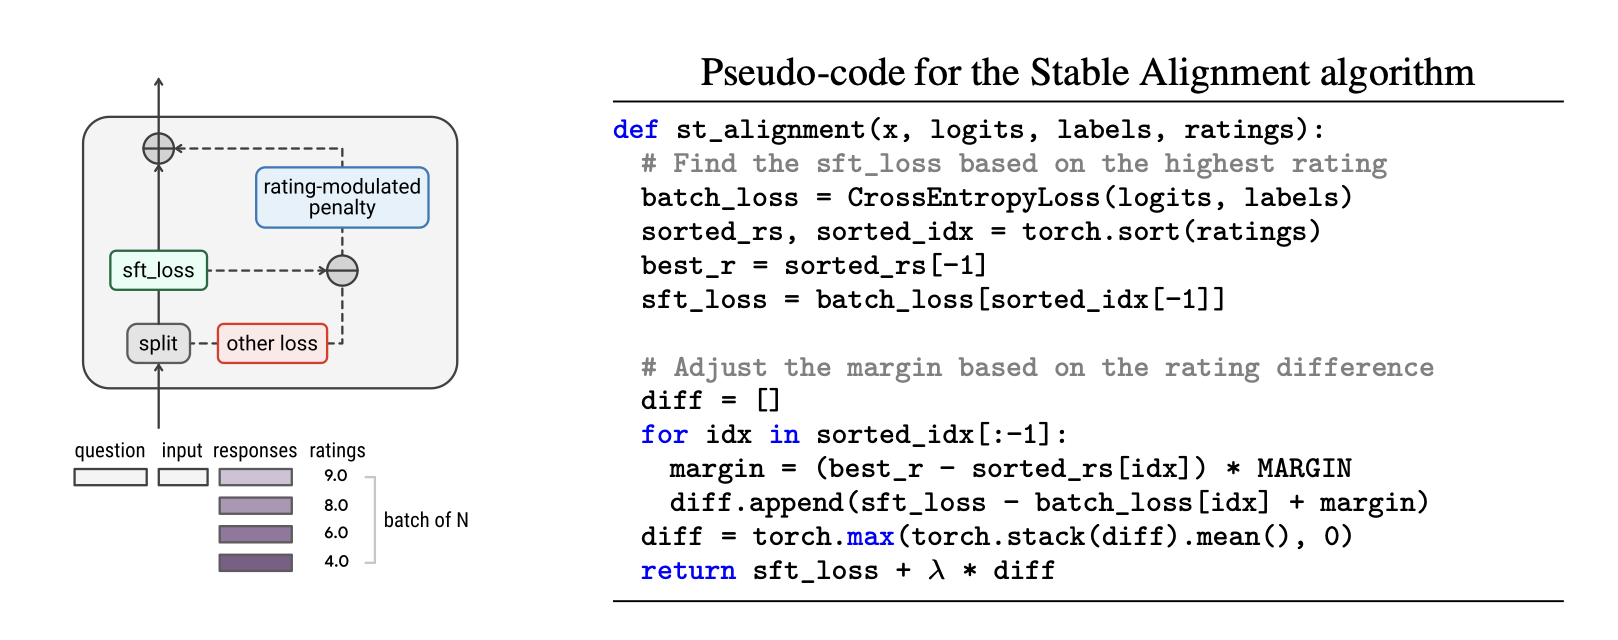
\includegraphics[width=\textwidth]{Liu2}
			\end{center}
		\end{frame}
		\begin{frame}
			\frametitle{Benchmarks}
			\begin{center}
				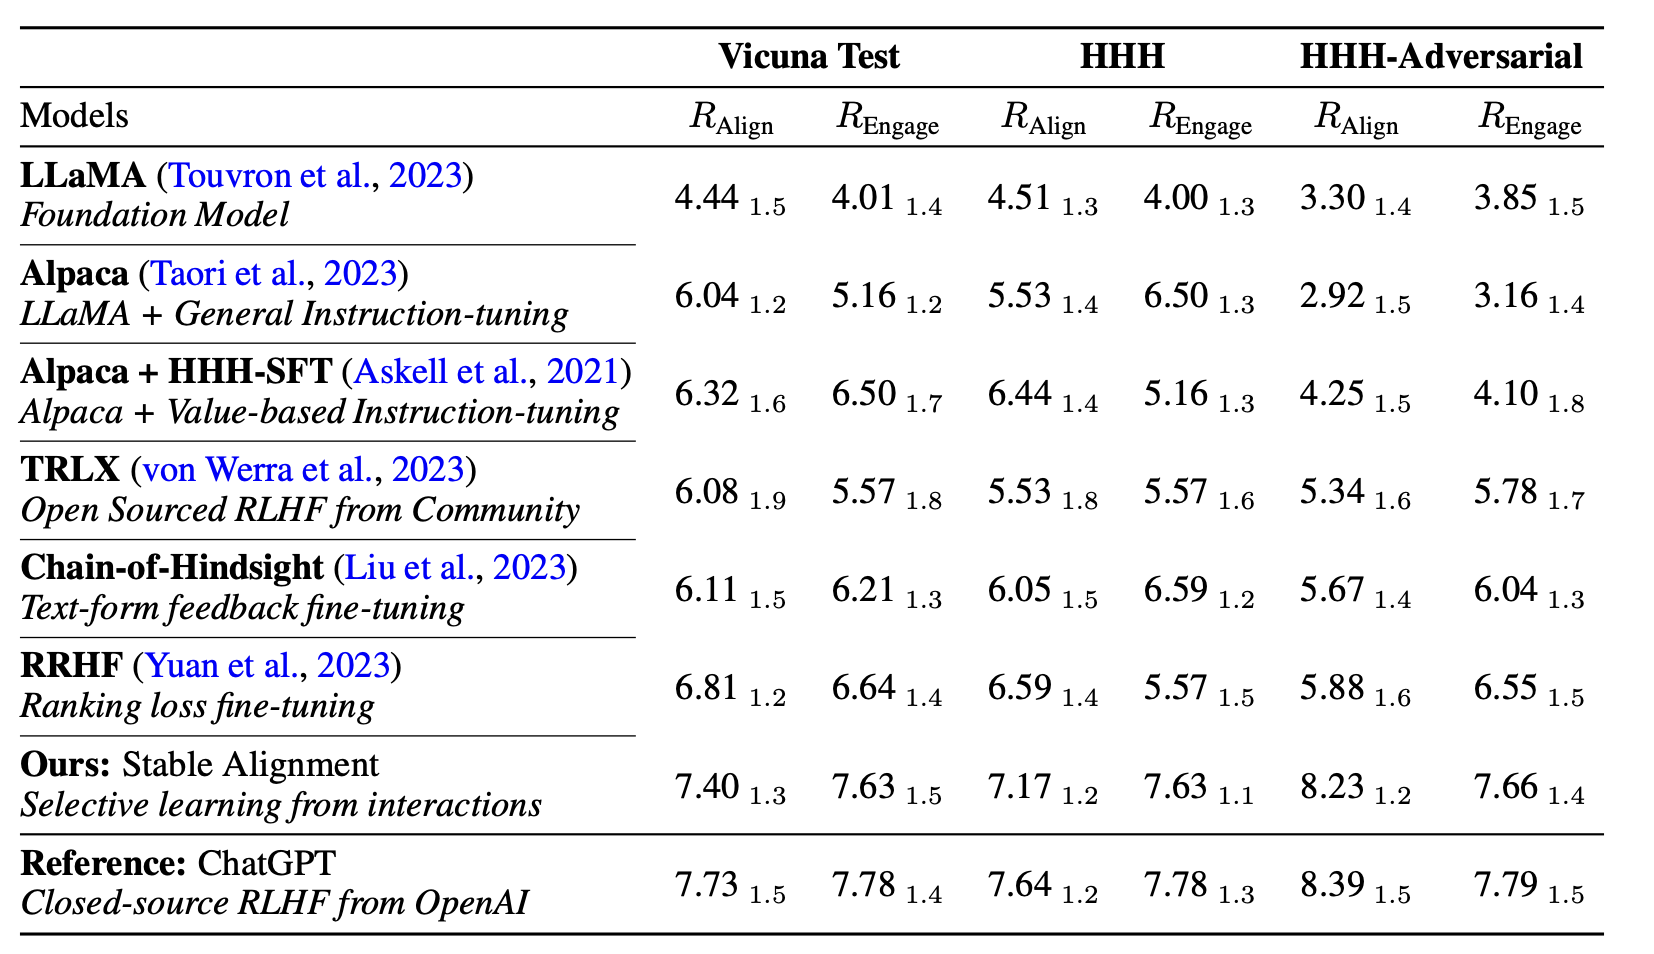
\includegraphics[width=\textwidth]{Liu3}
			\end{center}
		\end{frame}
		\begin{frame}
			\frametitle{Human evaluation}
			\begin{center}
				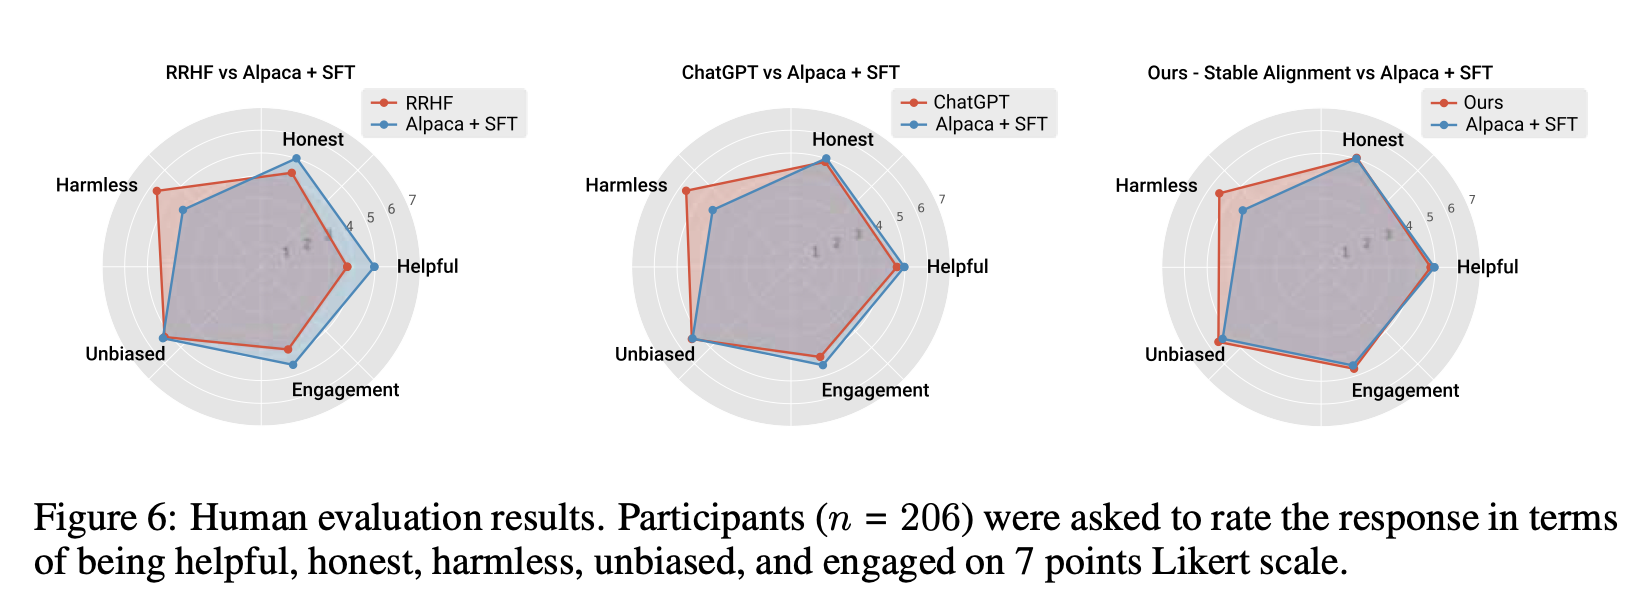
\includegraphics[width=\textwidth]{Liu4}
			\end{center}
		\end{frame}
		
	\section{ Gameplay with LLMs}
	\begin{frame}
		\frametitle{Title}
		\begin{center}
			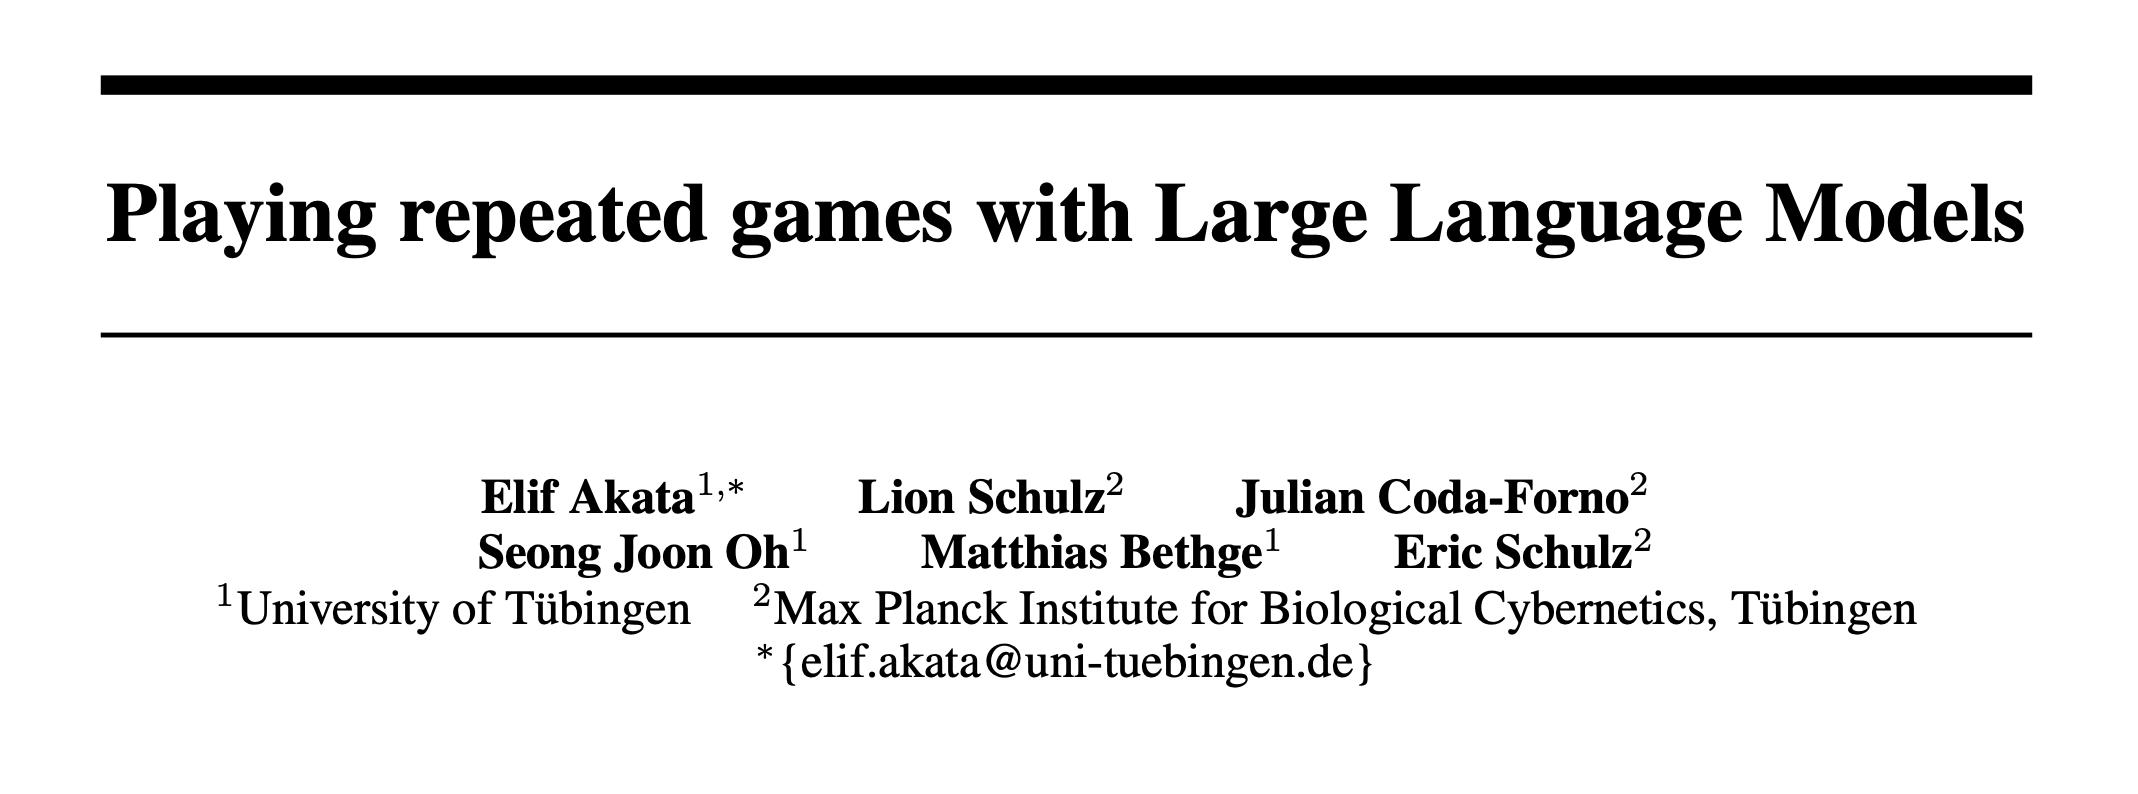
\includegraphics[width=\textwidth]{Akata0}
		\end{center}
	\end{frame}
	
	\begin{frame}
		\frametitle{Research Questions
		}
		\begin{itemize}
			\item How do LLMs behave when playing 2-player games with cooperation and coordination?
		\end{itemize}
	\end{frame}
	
	\begin{frame}
		\frametitle{Main Contributions
		}
		\begin{itemize}
			\item Behavioral analysis of LLMs (GPT3, 3.5, 4) across 2-player 2 action matrix games
			\item Including games with coordination and defection like Prisoner's dilemma and Battle of the Sexes
		\end{itemize}
	\end{frame}
	\begin{frame}
		\frametitle{General Framework}
		\begin{center}
			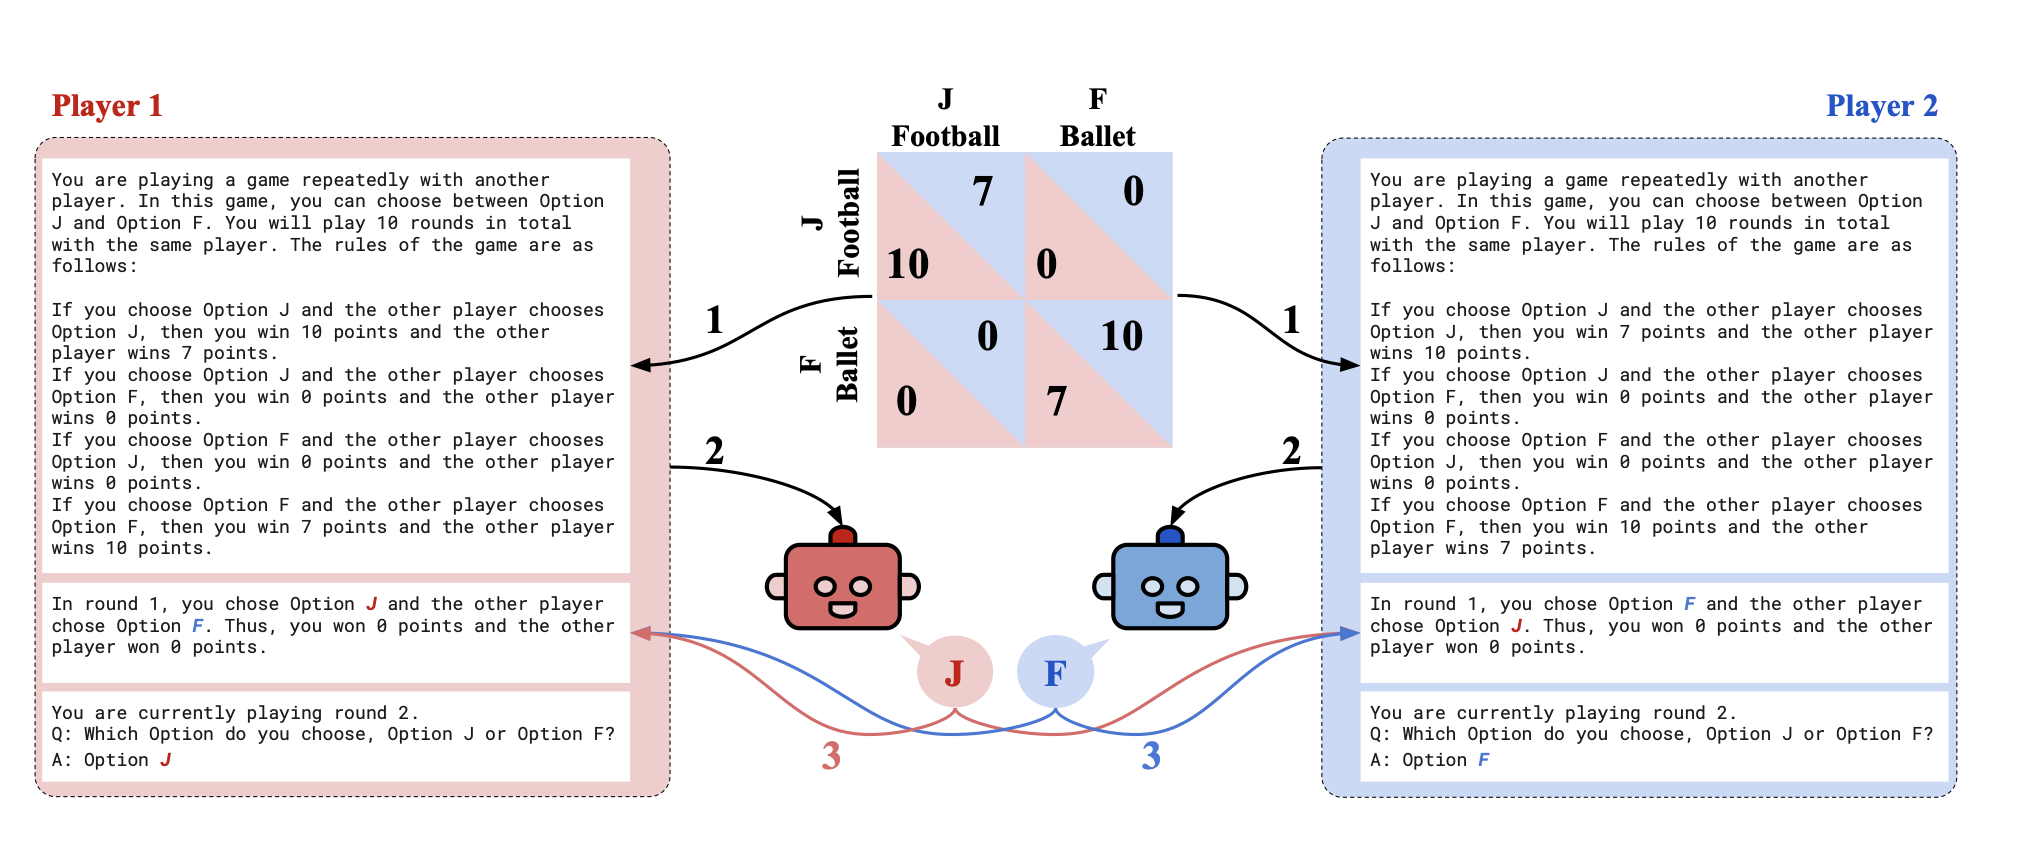
\includegraphics[width=\textwidth]{Akata1}
		\end{center}
	\end{frame}
	
	\begin{frame}
		\frametitle{Performance Across Families}
		\begin{center}
			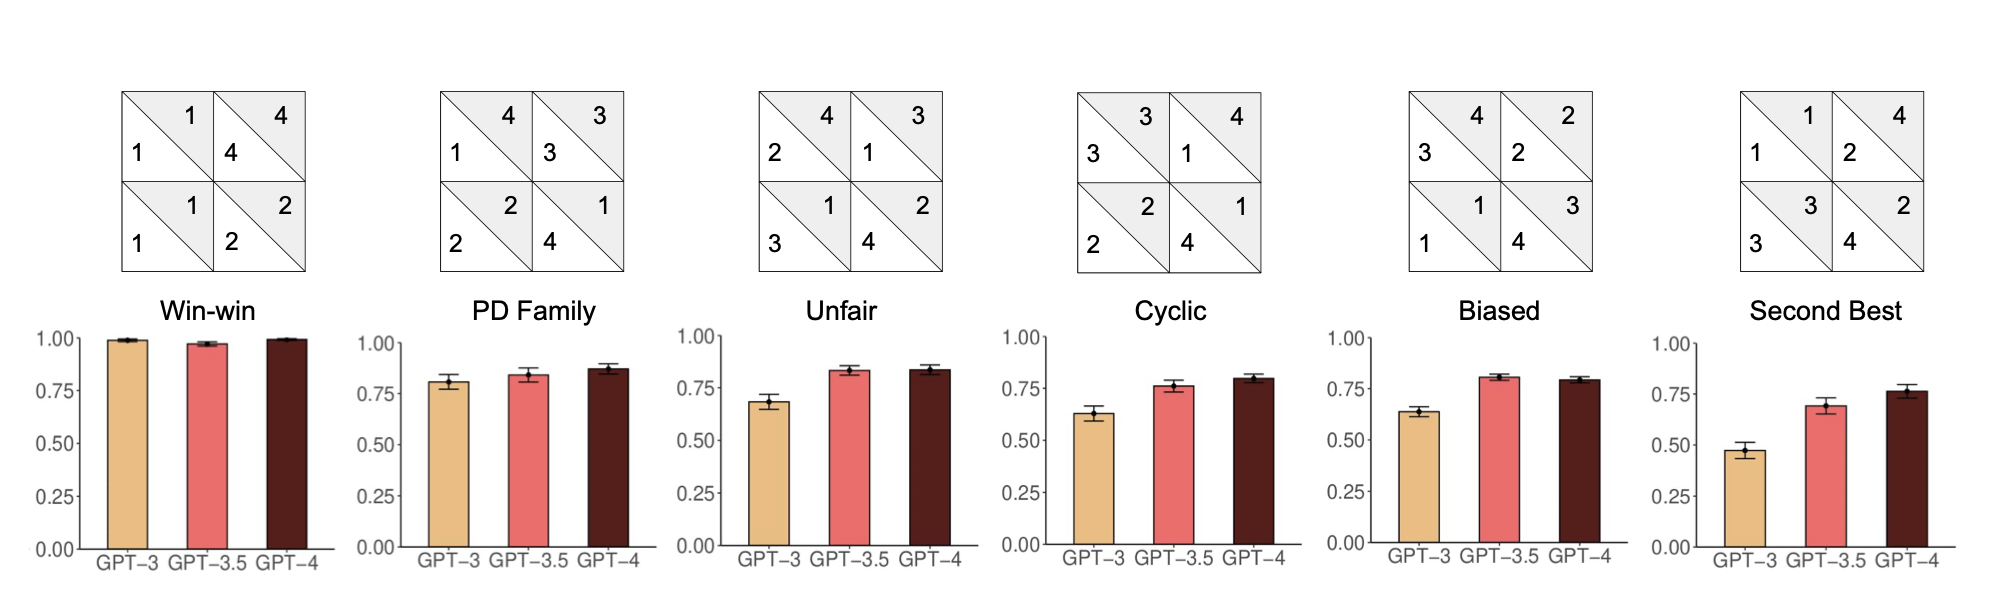
\includegraphics[width=\textwidth]{Akata2}
		\end{center}
	\end{frame}
	
	\begin{frame}
		\frametitle{Prisoner's Dilemma Defection}
		\begin{center}
			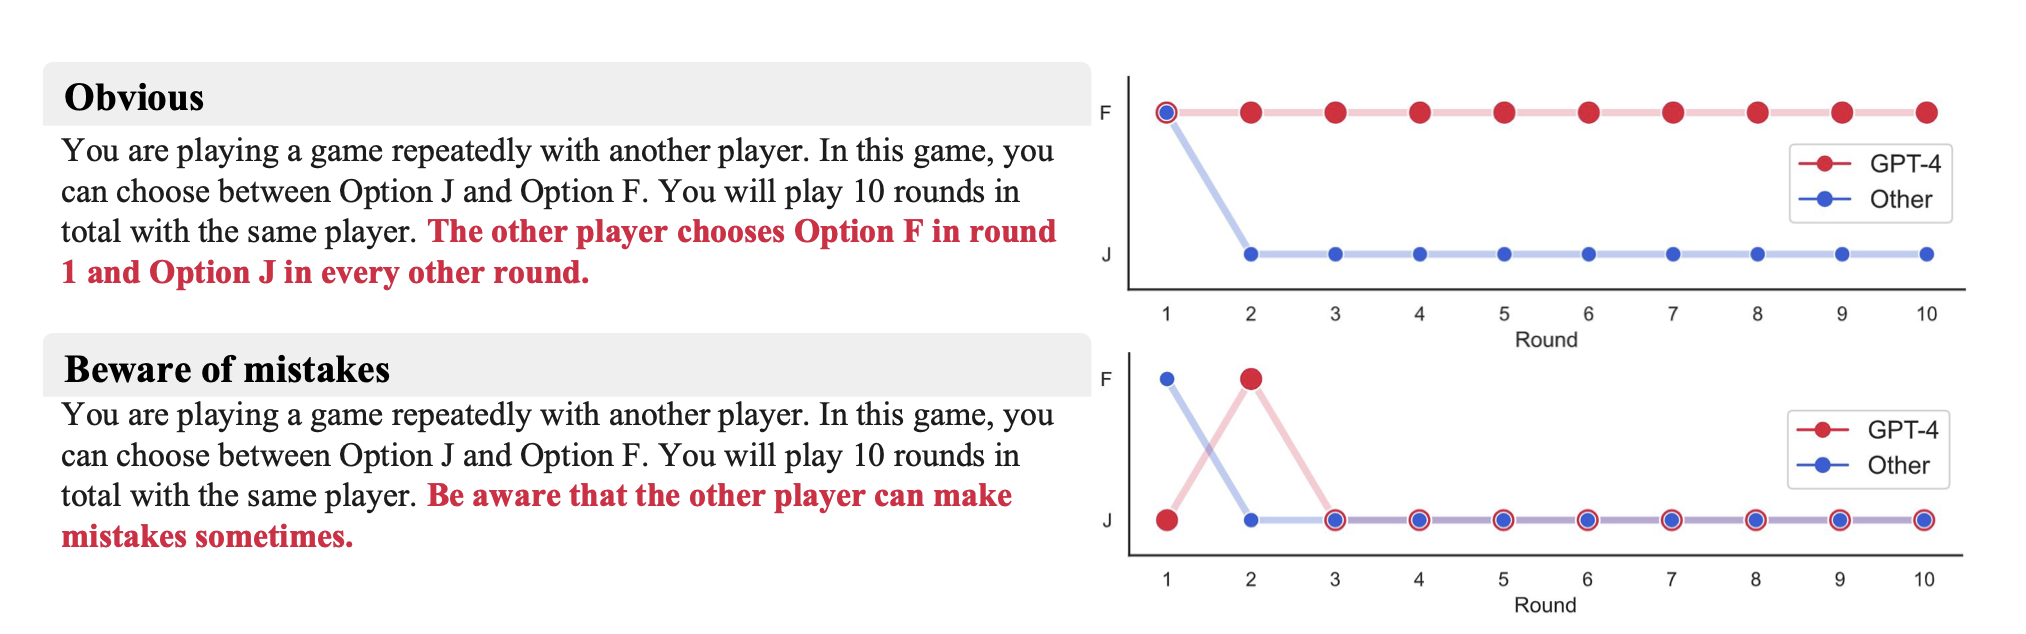
\includegraphics[width=\textwidth]{Akata3}
		\end{center}
	\end{frame}
	
	\begin{frame}
		\frametitle{Battle of the Sexes Coordination}
		\begin{center}
			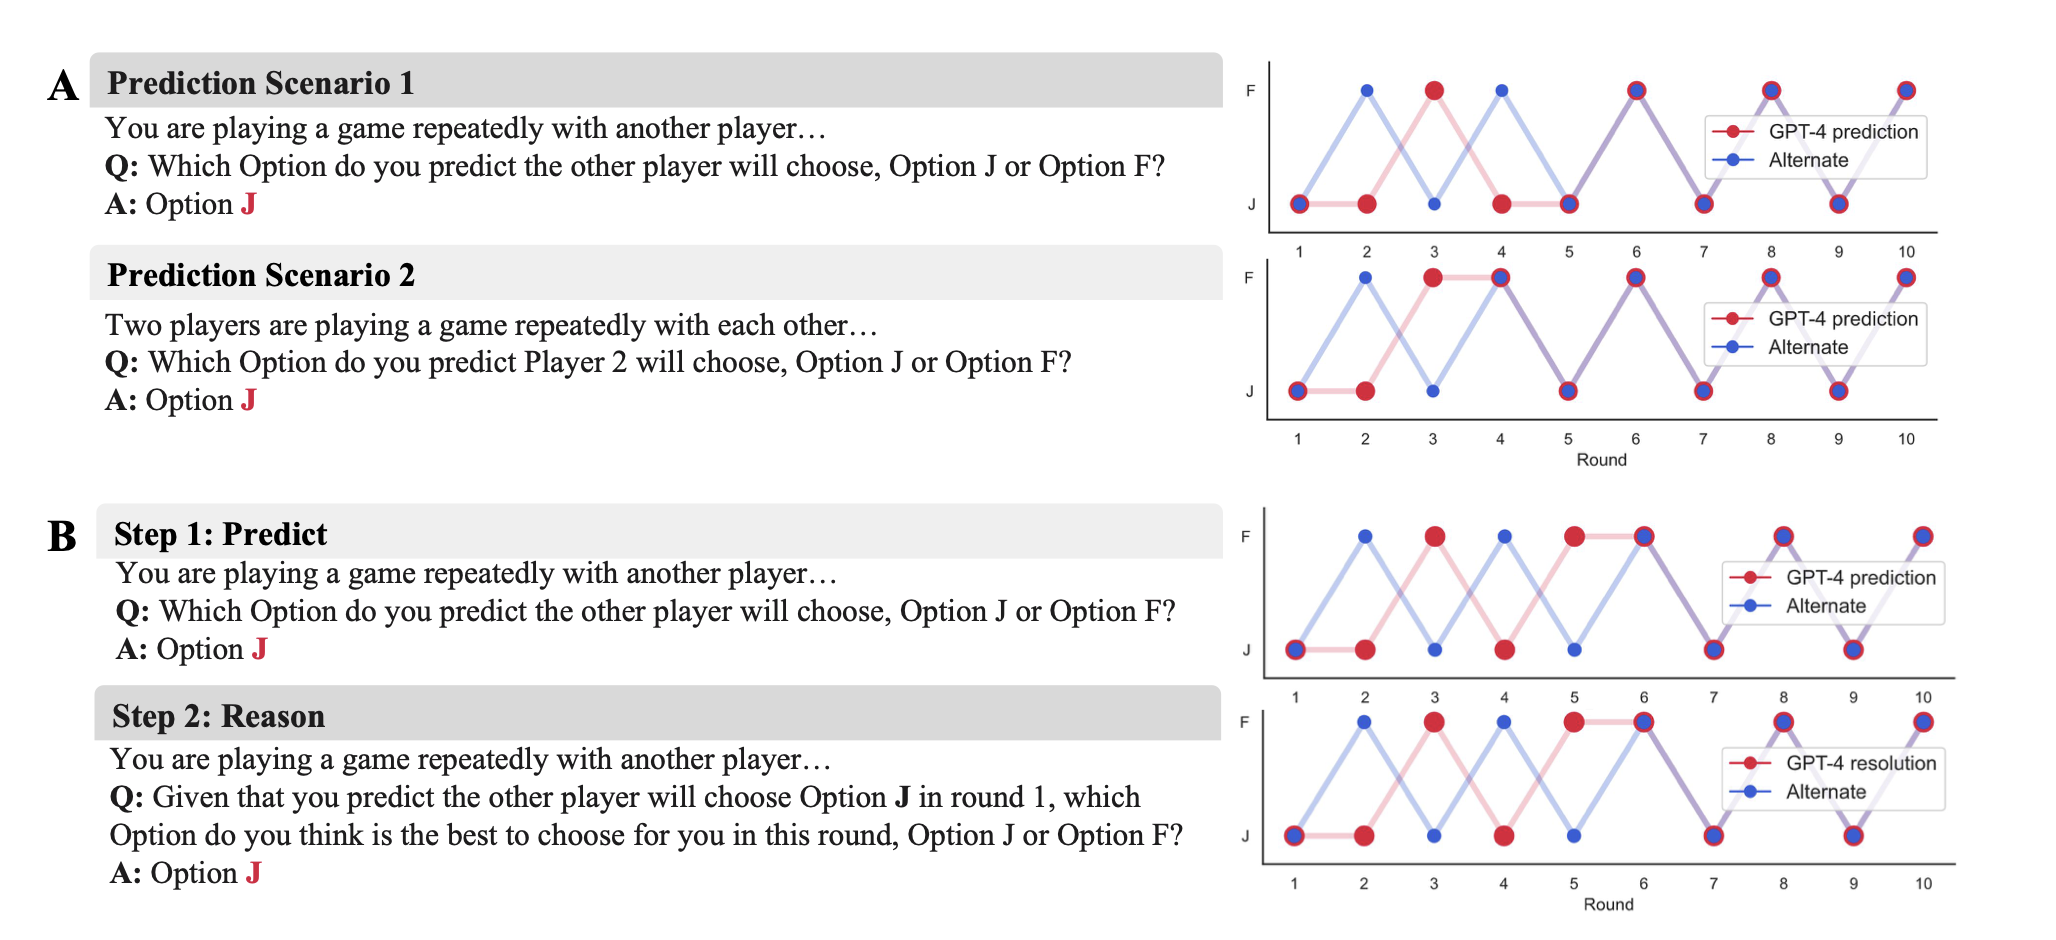
\includegraphics[width=\textwidth]{Akata4}
		\end{center}
	\end{frame}
	
%	\section{Repeated Gameplay with LLMs}
%\begin{frame}
%\frametitle{Title}
%\begin{center}
%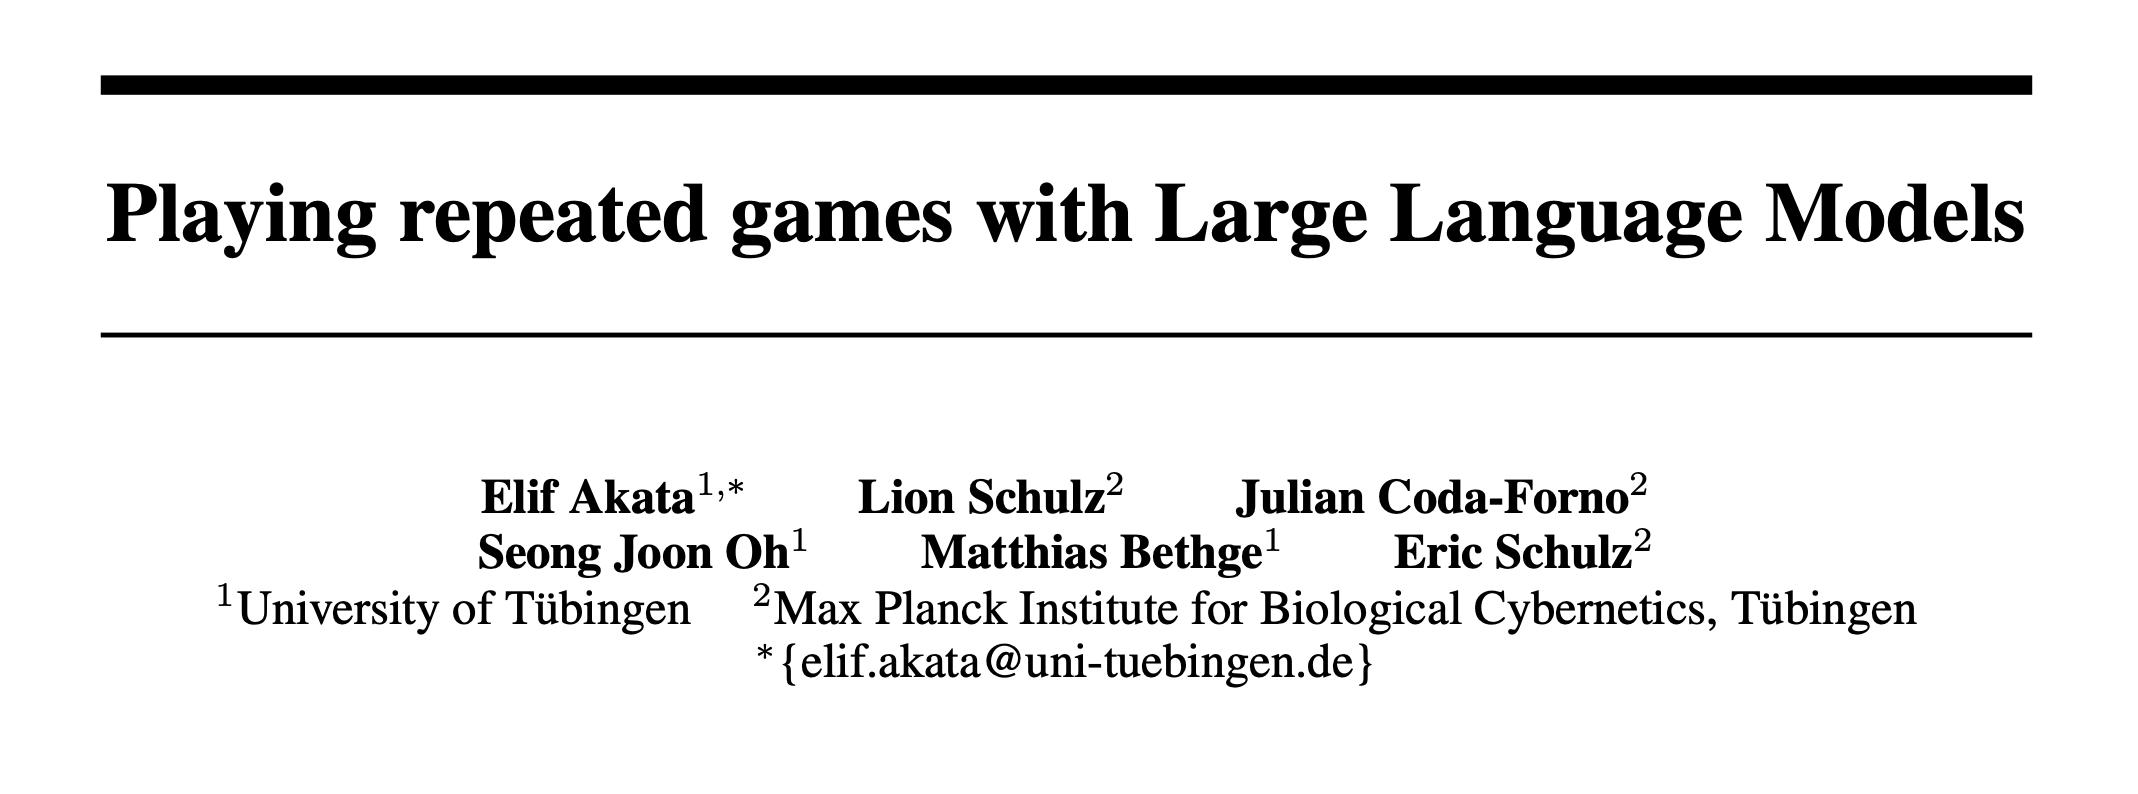
\includegraphics[width=\textwidth]{Akata0}
%\end{center}
%\end{frame}
%
%\begin{frame}
%\frametitle{Research Questions
%}
%\begin{itemize}
%\item How do LLMs behave when playing 2-player games with cooperation and coordination?
%\end{itemize}
%\end{frame}
%
%\begin{frame}
%\frametitle{Main Contributions
%}
%\begin{itemize}
%\item Behavioral analysis of LLMs (GPT3, 3.5, 4) across 2-player 2 action matrix games
%\item Including games with coordination and defection like Prisoner's dilemma and Battle of the Sexes
%\end{itemize}
%\end{frame}
%\begin{frame}
%\frametitle{General Framework}
%\begin{center}
%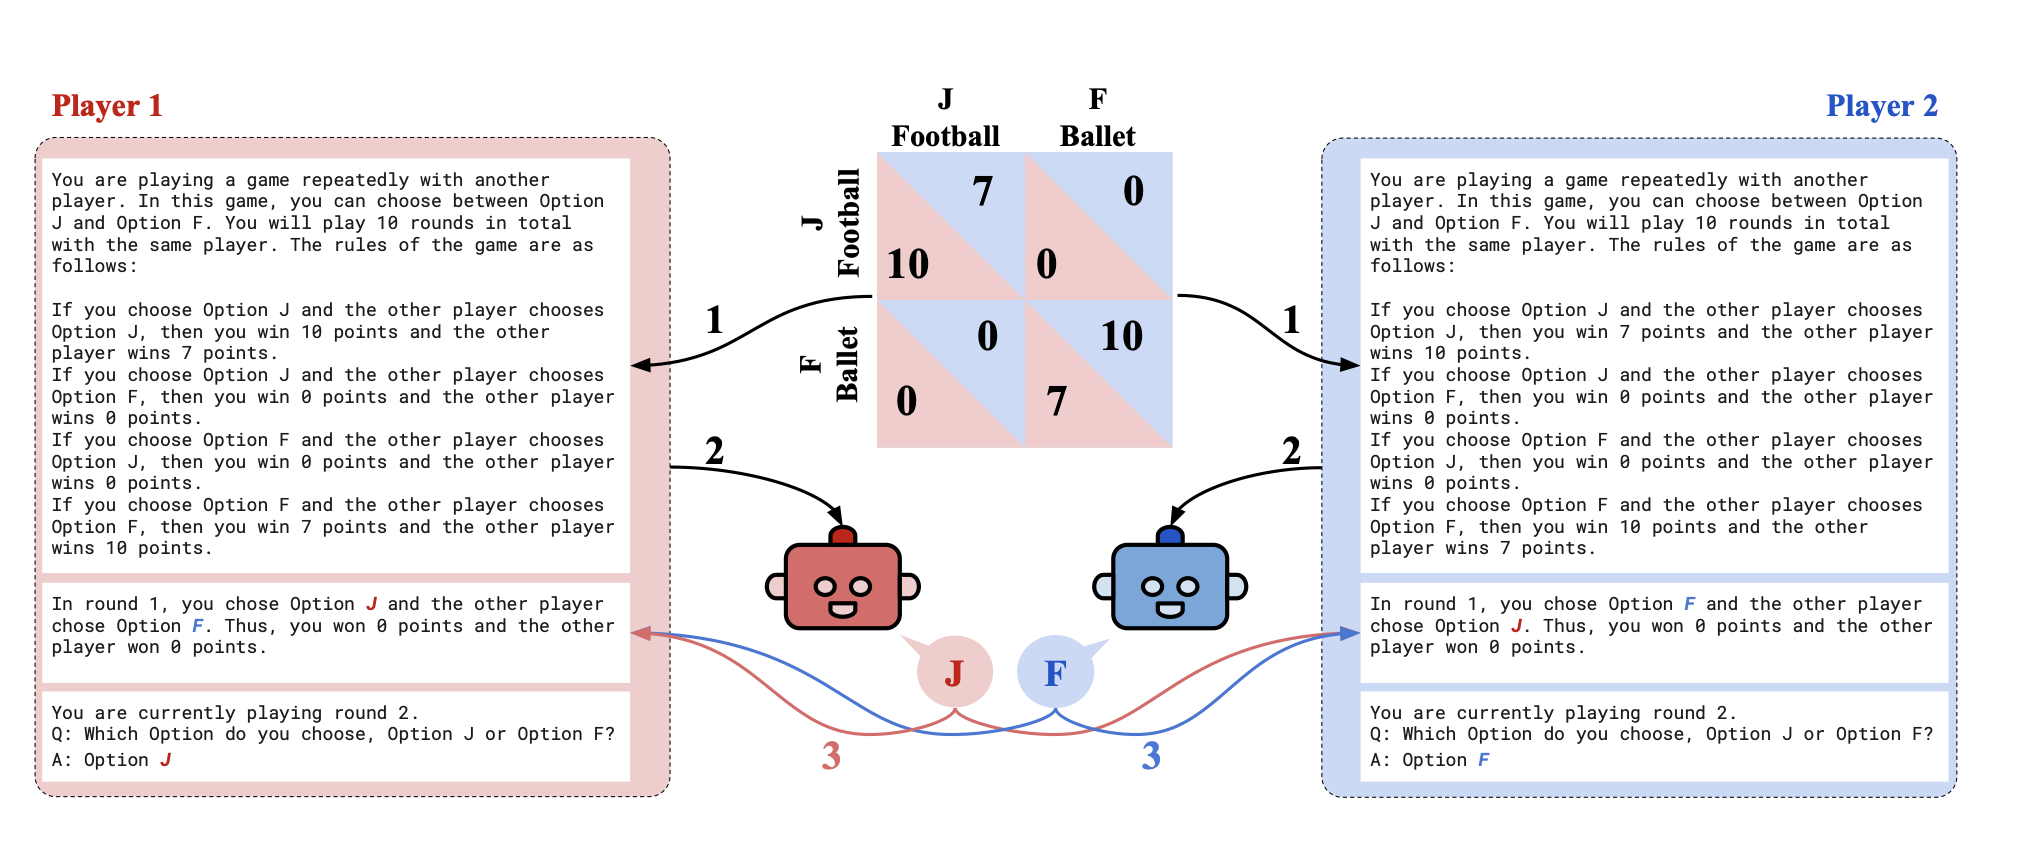
\includegraphics[width=\textwidth]{Akata1}
%\end{center}
%\end{frame}
%
%\begin{frame}
%\frametitle{Performance Across Families}
%\begin{center}
%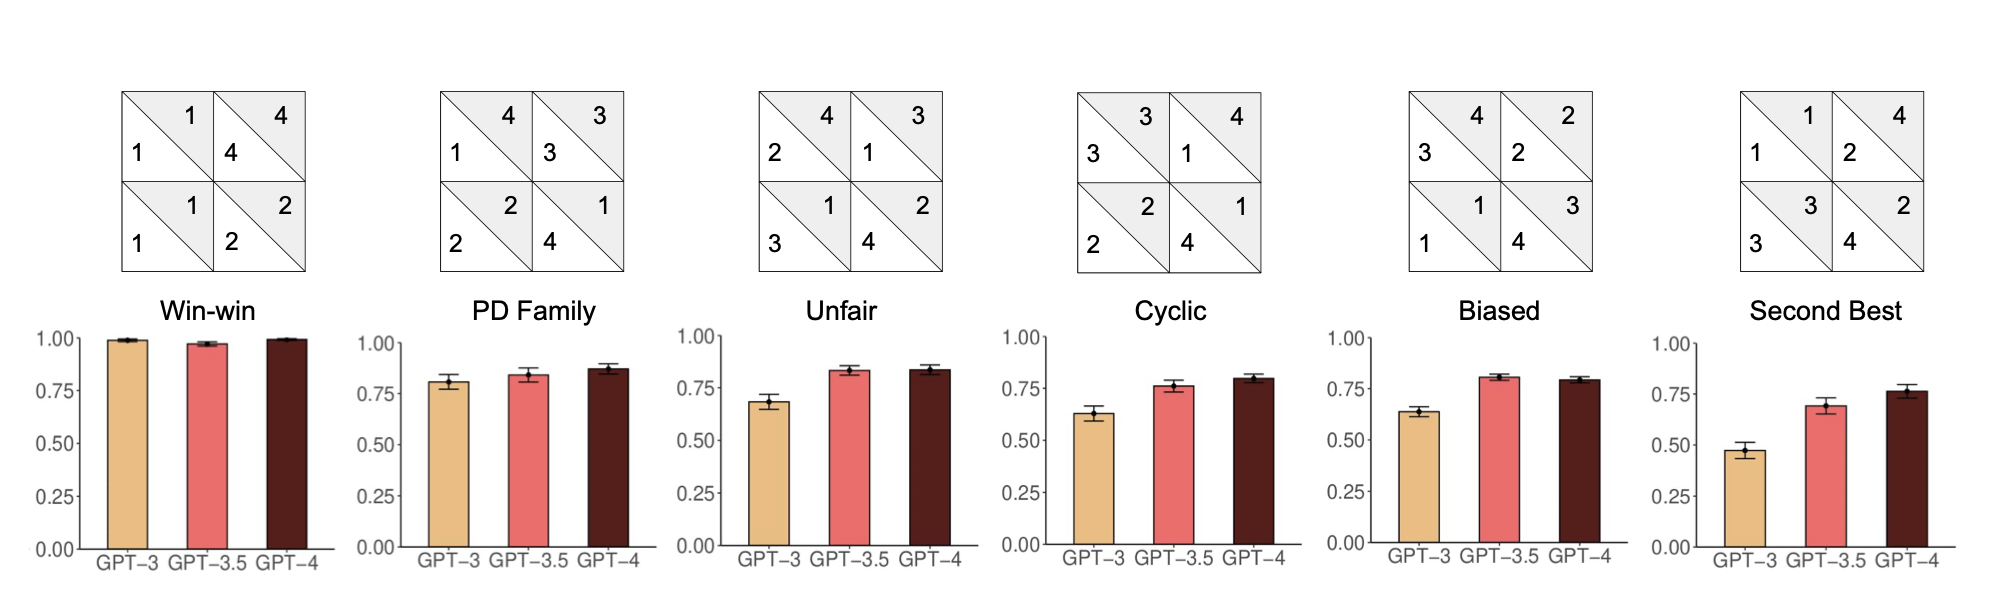
\includegraphics[width=\textwidth]{Akata2}
%\end{center}
%\end{frame}
%
%\begin{frame}
%\frametitle{Prisoner's Dilemma Defection}
%\begin{center}
%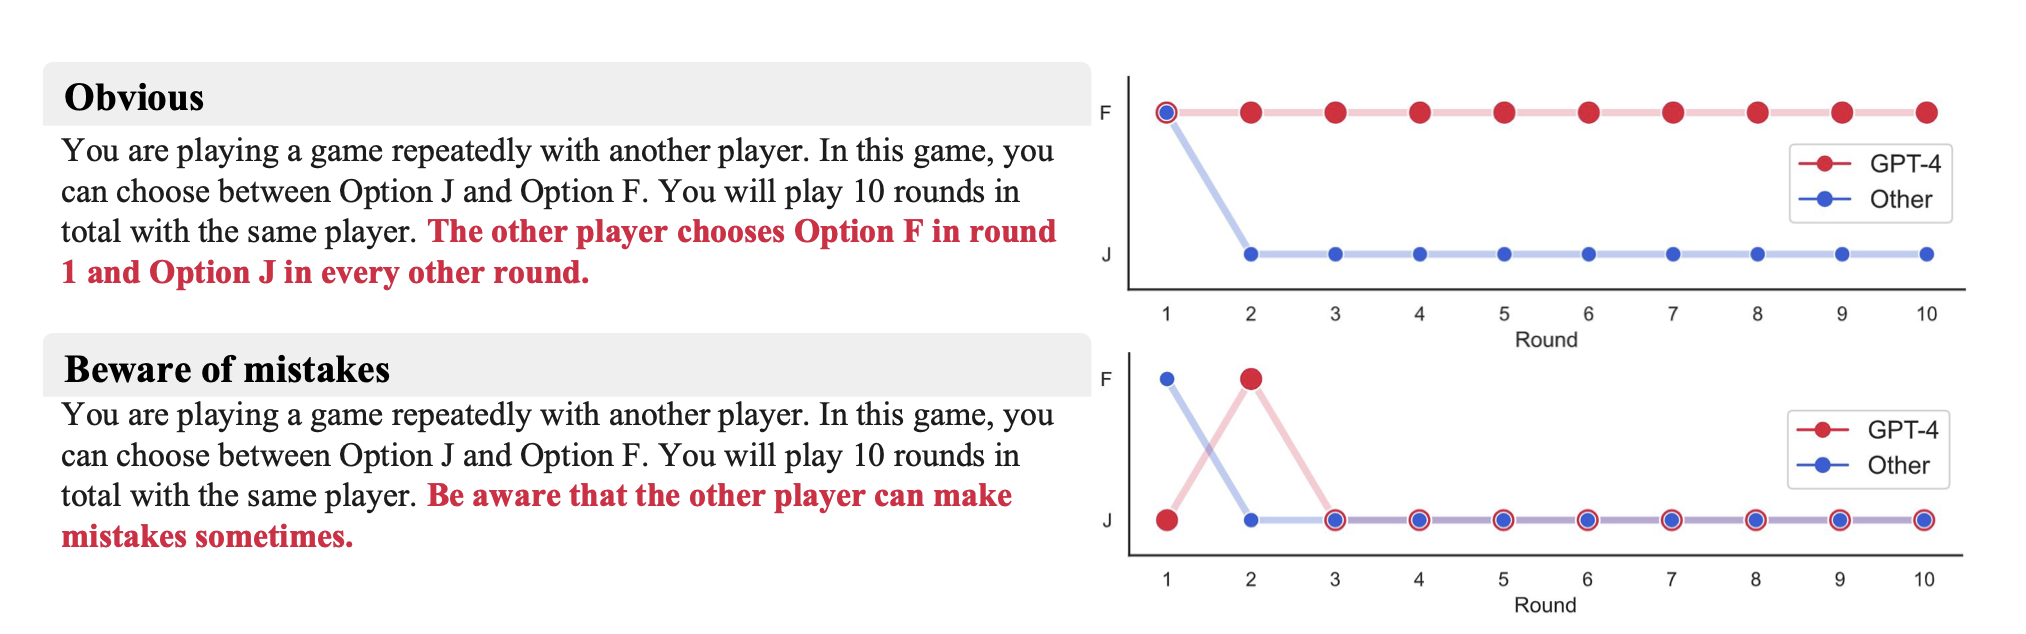
\includegraphics[width=\textwidth]{Akata3}
%\end{center}
%\end{frame}
%
%\begin{frame}
%\frametitle{Battle of the Sexes Coordination}
%\begin{center}
%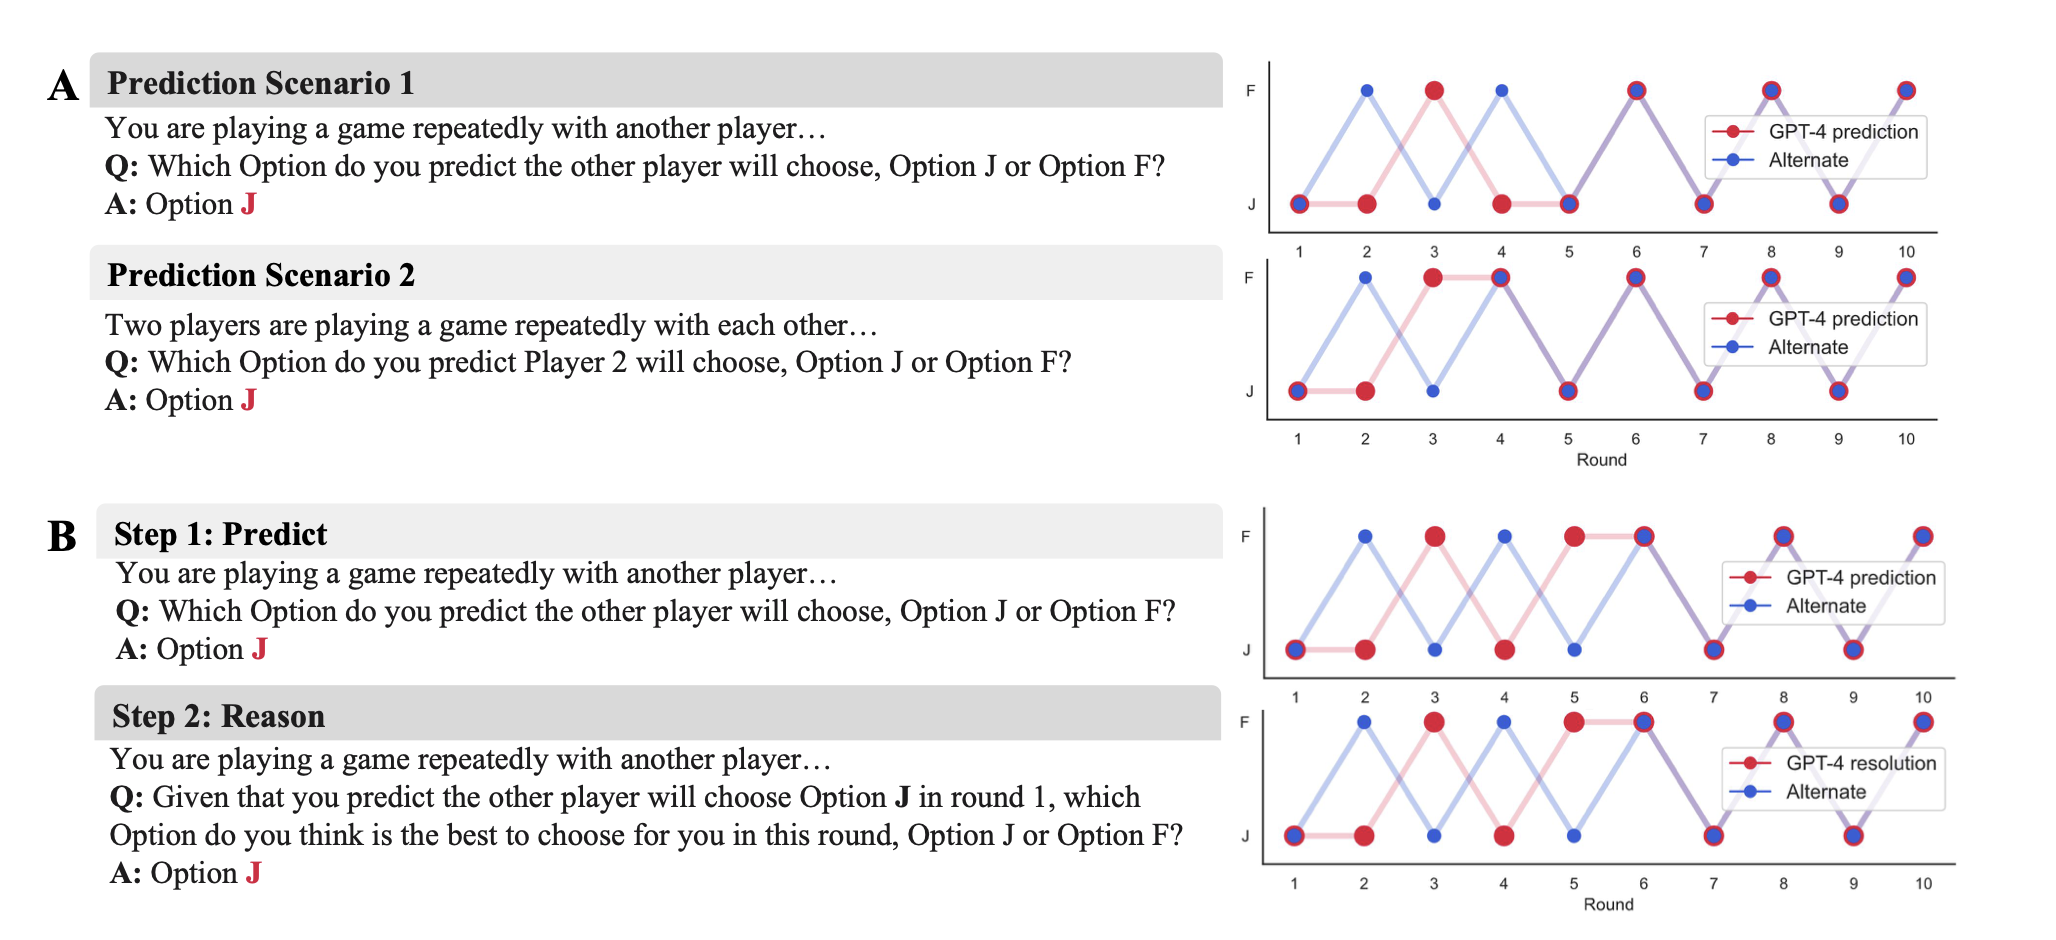
\includegraphics[width=\textwidth]{Akata4}
%\end{center}
%\end{frame}

%\section{InstructGPT}
%	\begin{frame}
%		\frametitle{Title}
%		\begin{center}
%			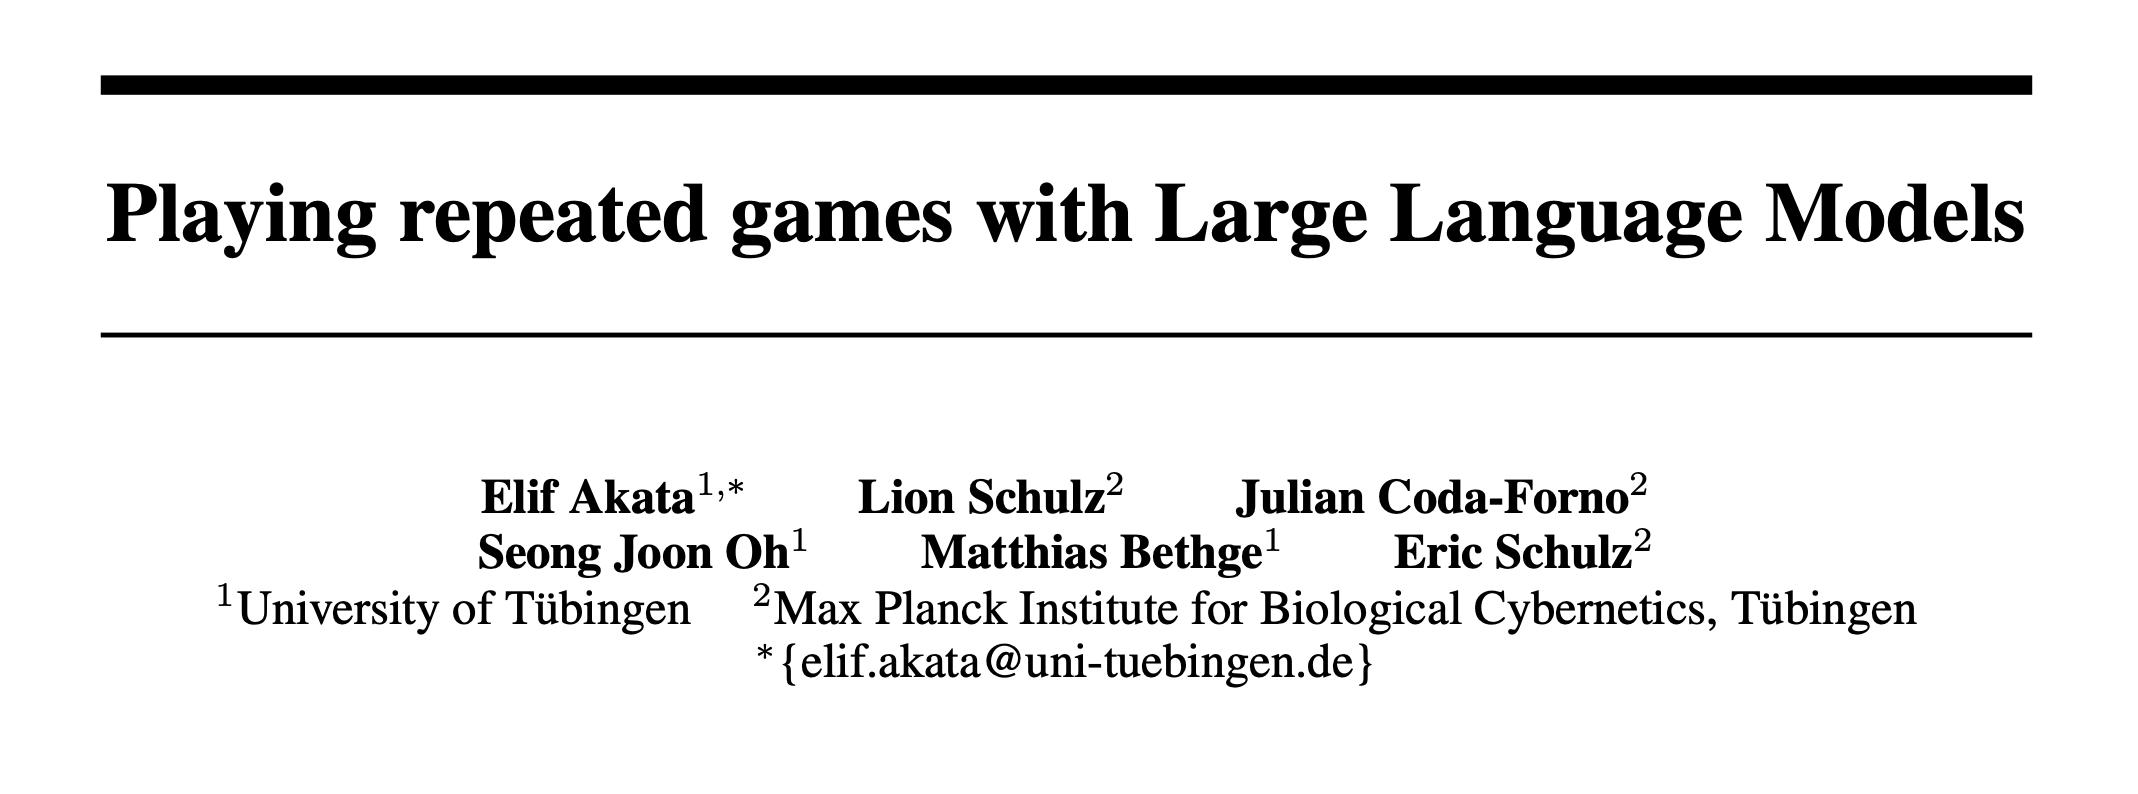
\includegraphics[width=\textwidth]{Akata0}
%		\end{center}
%	\end{frame}
%	
%	\begin{frame}
%		\frametitle{Research Questions
%		}
%		\begin{itemize}
%			\item How do LLMs behave when playing 2-player games with cooperation and coordination?
%		\end{itemize}
%	\end{frame}
%	
%	\begin{frame}
%		\frametitle{Main Contributions
%		}
%		\begin{itemize}
%			\item Behavioral analysis of LLMs (GPT3, 3.5, 4) across 2-player 2 action matrix games
%			\item Including games with coordination and defection like Prisoner's dilemma and Battle of the Sexes
%		\end{itemize}
%	\end{frame}
%	\begin{frame}
%		\frametitle{General Framework}
%		\begin{center}
%			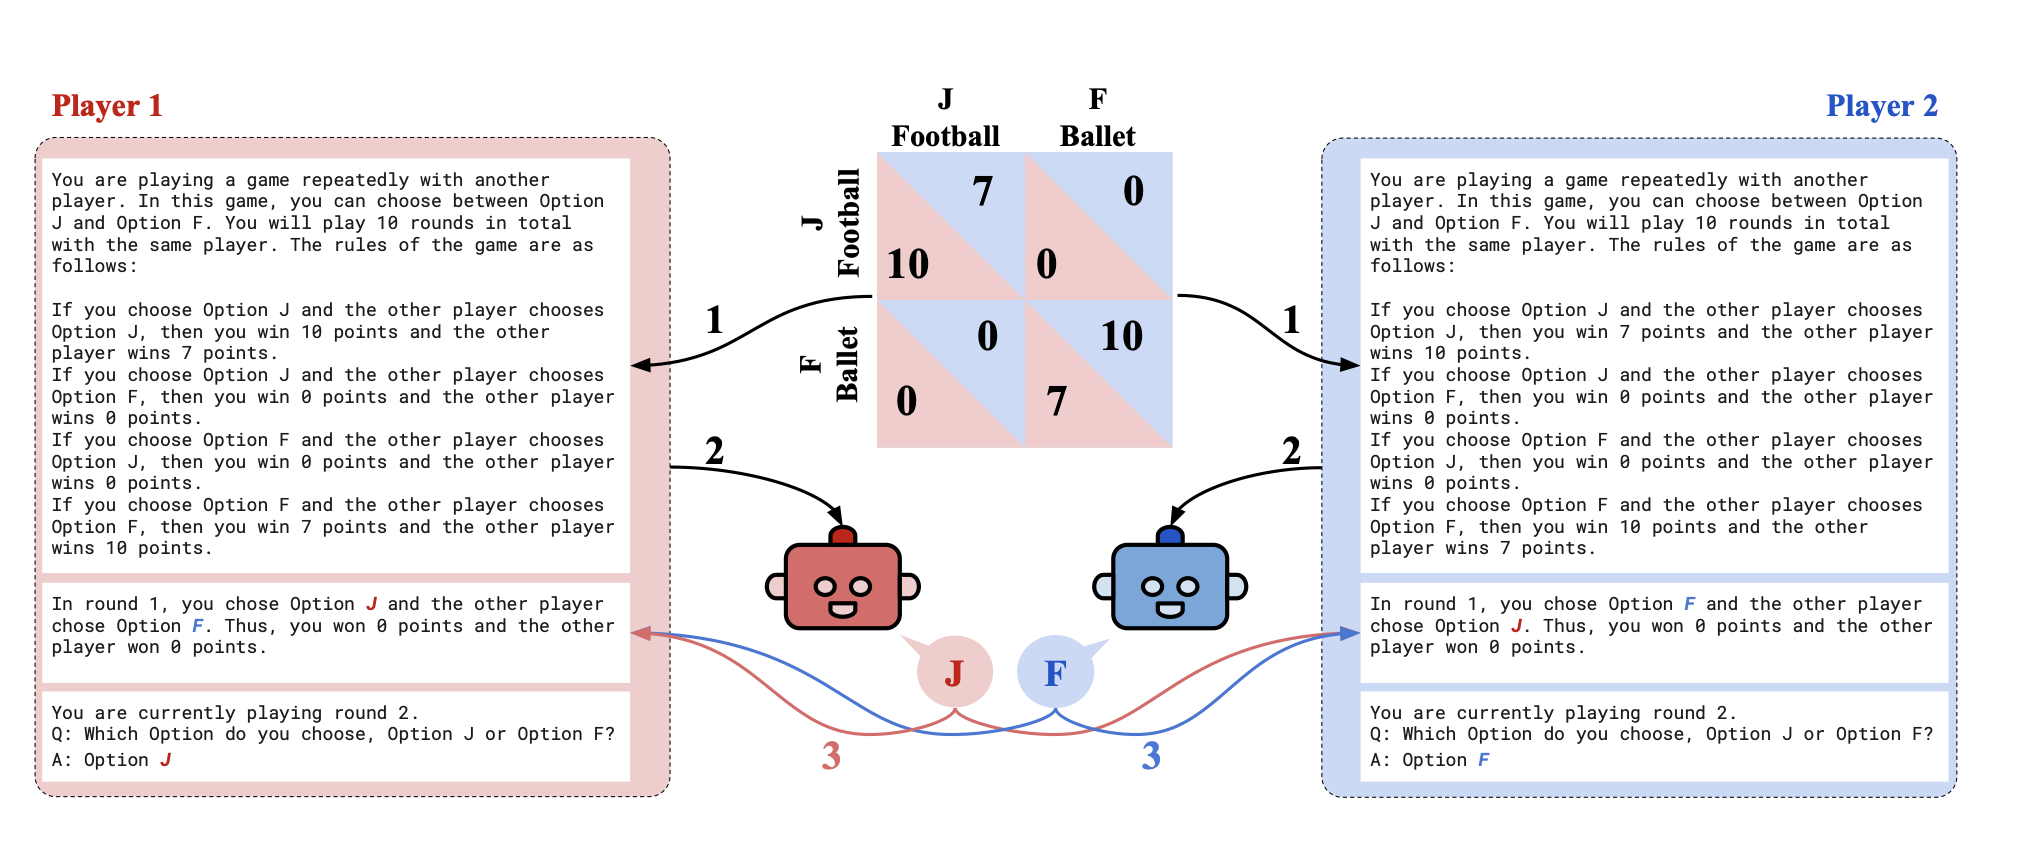
\includegraphics[width=\textwidth]{Akata1}
%		\end{center}
%	\end{frame}


\section{Self-Instruct}
\begin{frame}
	\frametitle{Title}
	\begin{center}
		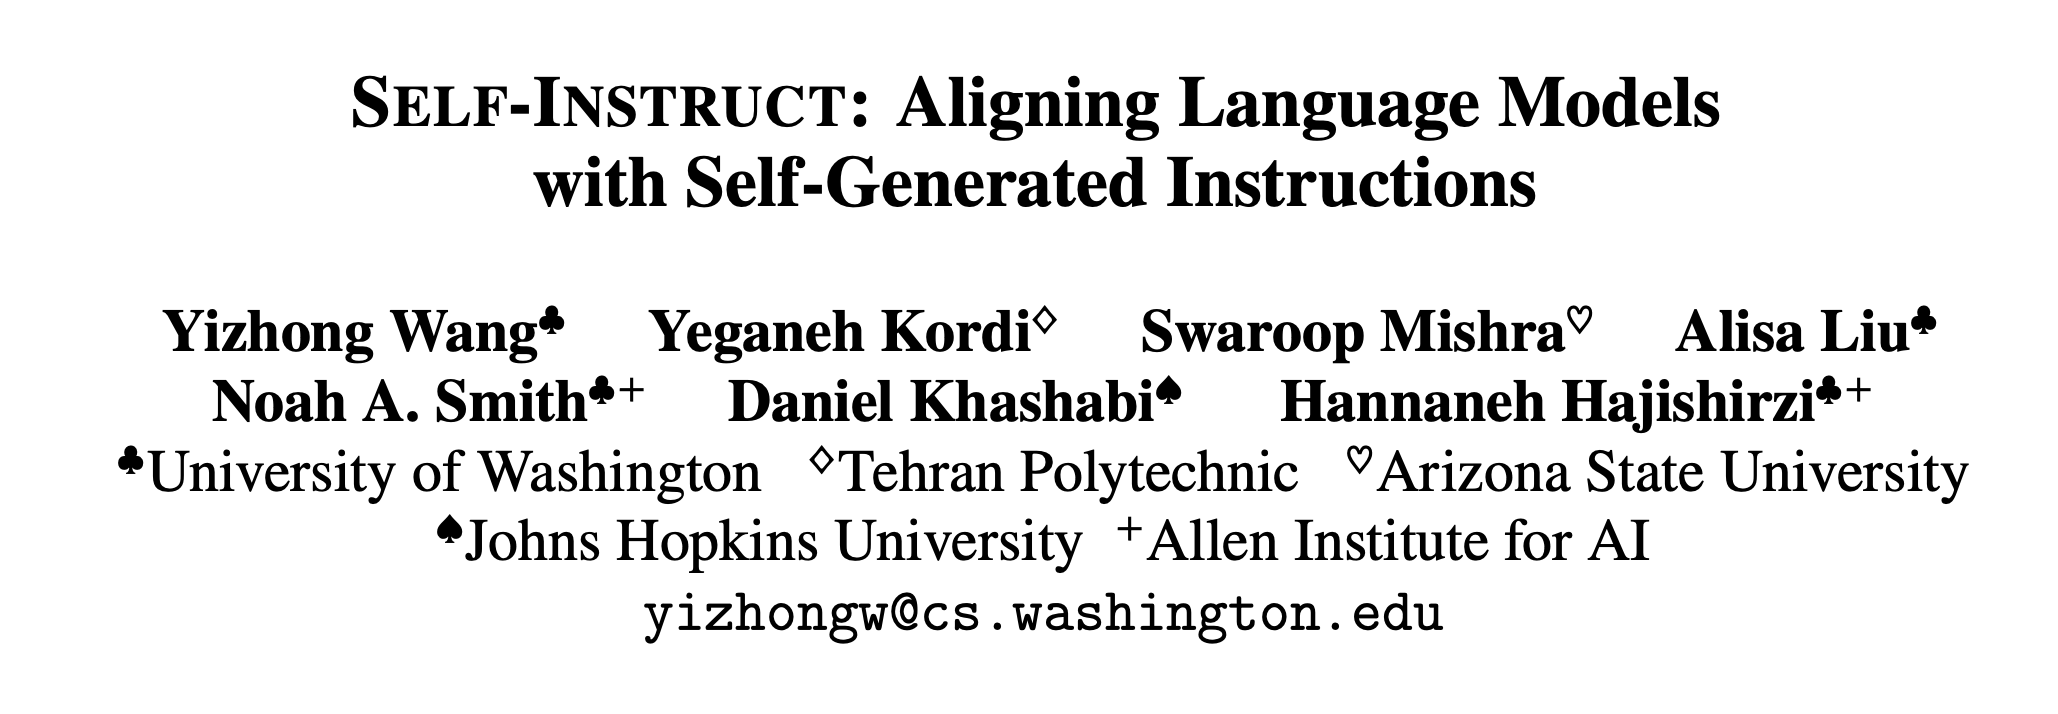
\includegraphics[width=\textwidth]{Wang0}
	\end{center}
\end{frame}

\begin{frame}
	\frametitle{Research Questions
	}
	\begin{itemize}
		\item How can we align LLMs effective and sample efficiently to following instructions?
	\end{itemize}
\end{frame}

\begin{frame}
	\frametitle{Main Contributions
	}
	\begin{itemize}
		\item Introduced method for generating more instructions and instruction following capabilities from minimal human-labeled data
		\item Demonstrated effectiveness using instruction-tuning experiments
		\item Generated new instruction dataset
	\end{itemize}
\end{frame}
\begin{frame}
	\frametitle{Example instructions}
	\begin{center}
		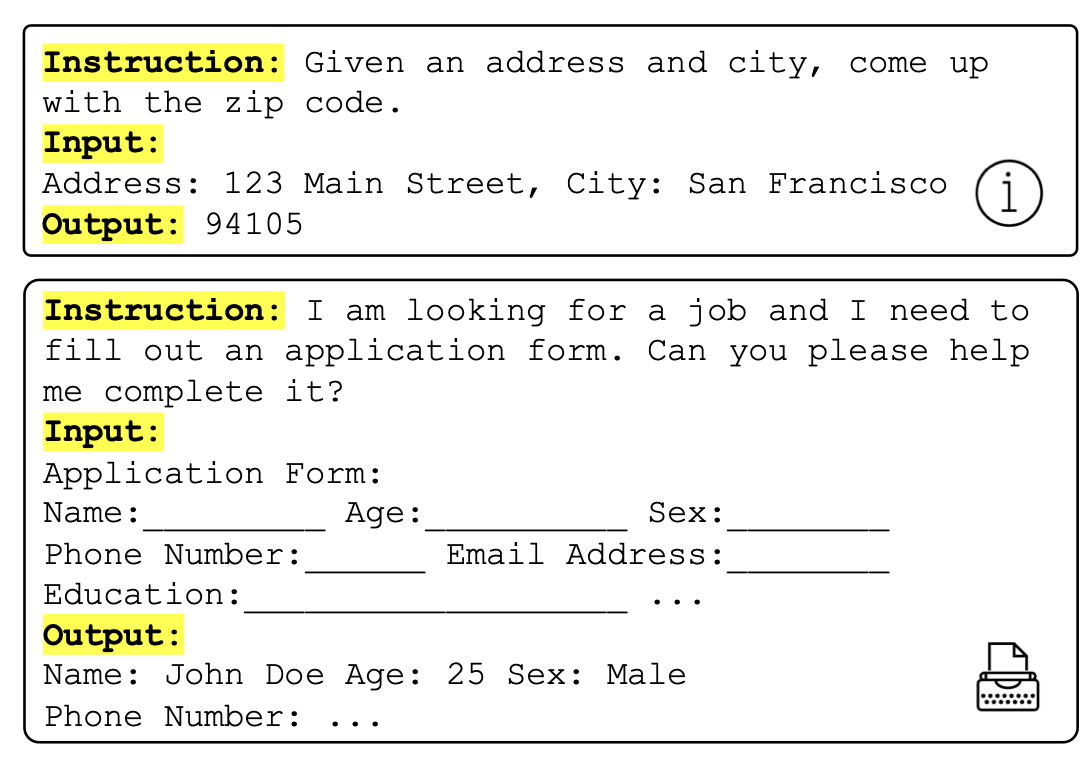
\includegraphics[scale=0.4]{Wang1}
	\end{center}
\end{frame}
\begin{frame}
	\frametitle{General Framework}
	\begin{center}
		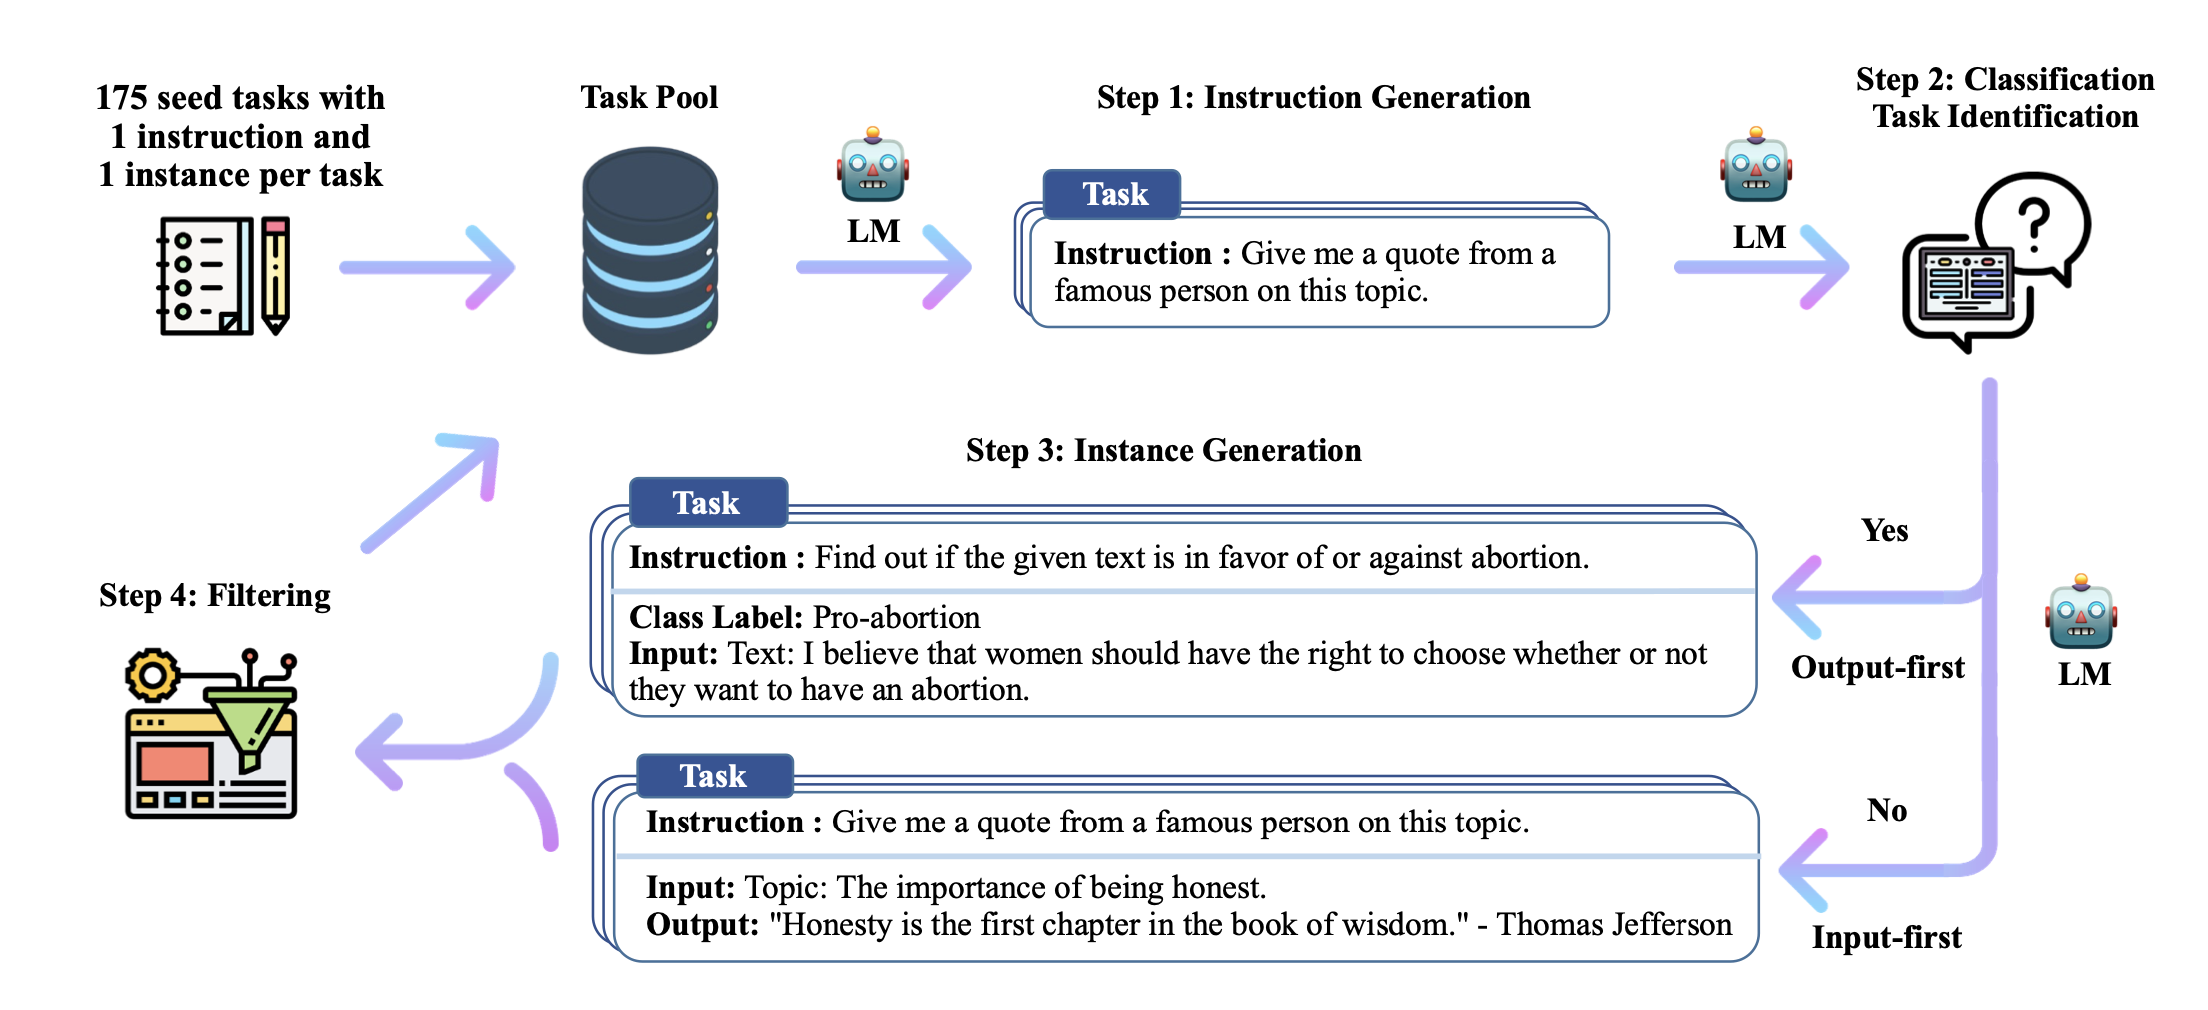
\includegraphics[width=\textwidth]{Wang2}
	\end{center}
\end{frame}
\begin{frame}
	\frametitle{Instruction Distribution}
	\begin{center}
		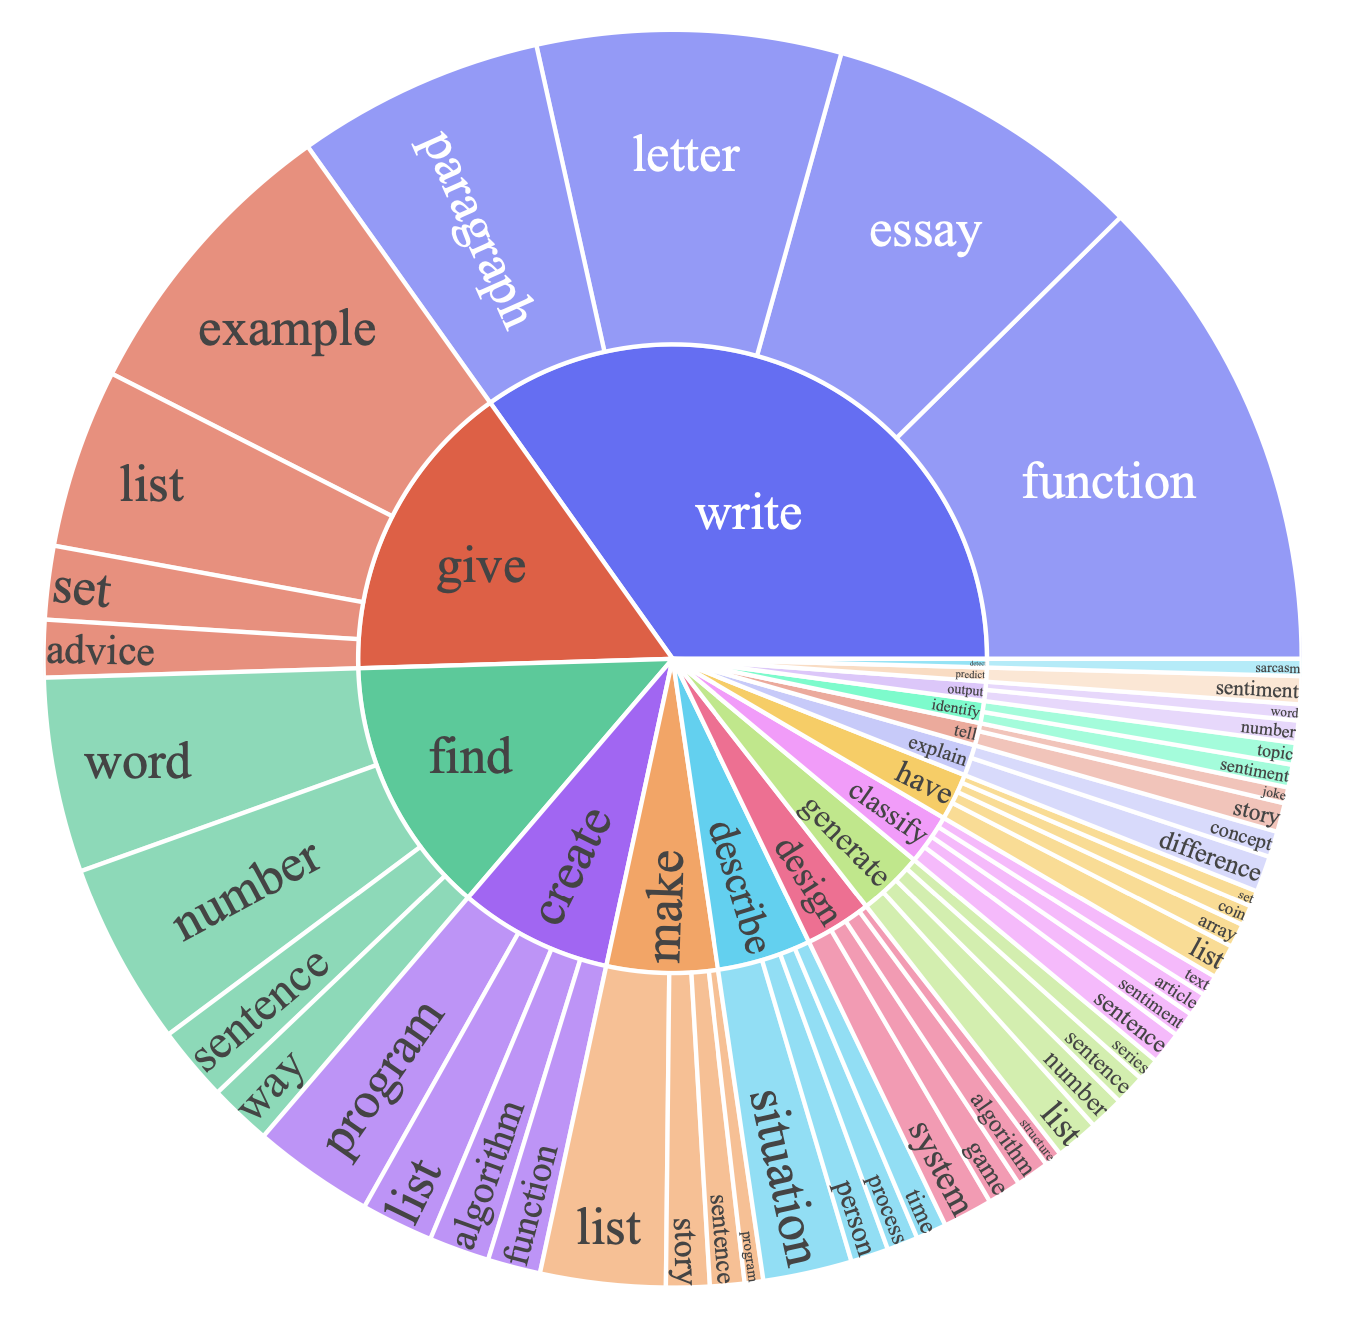
\includegraphics[scale=0.3]{Wang3}
	\end{center}
\end{frame}
\begin{frame}
	\frametitle{Performance}
	\begin{center}
		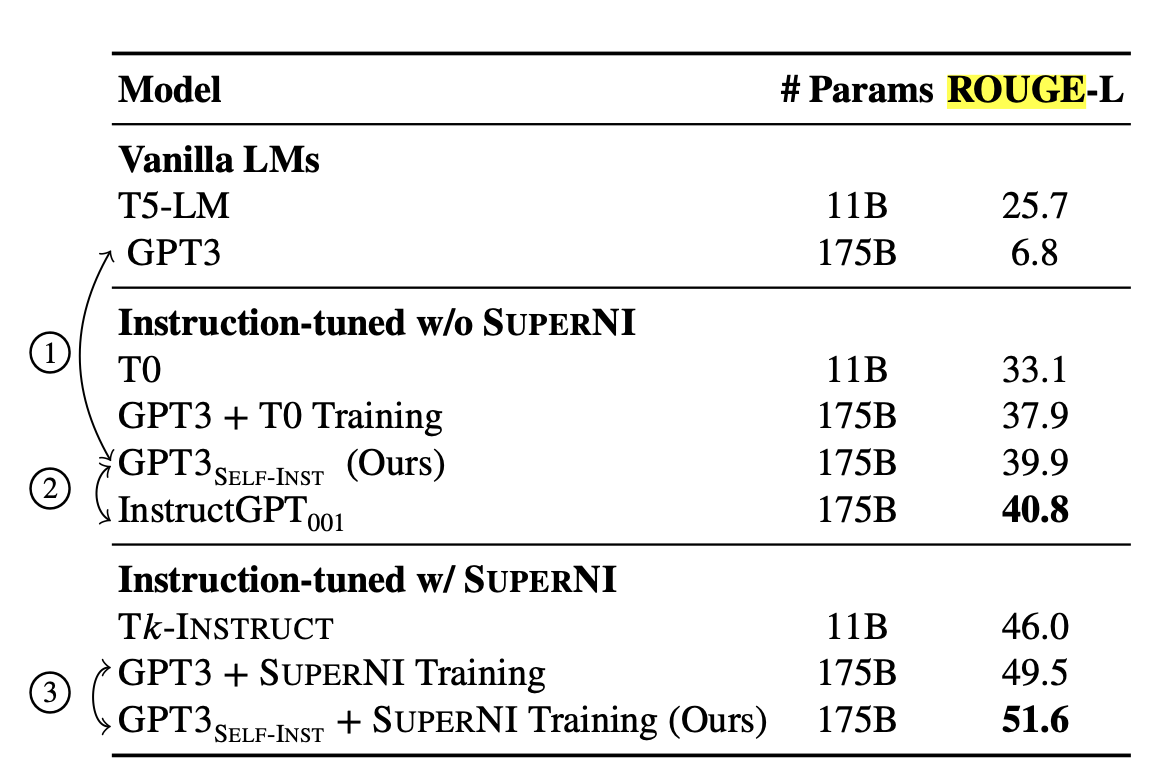
\includegraphics[scale=0.4]{Wang4}
	\end{center}
\end{frame}
\begin{frame}
	\frametitle{Human evaluation}
	\begin{center}
		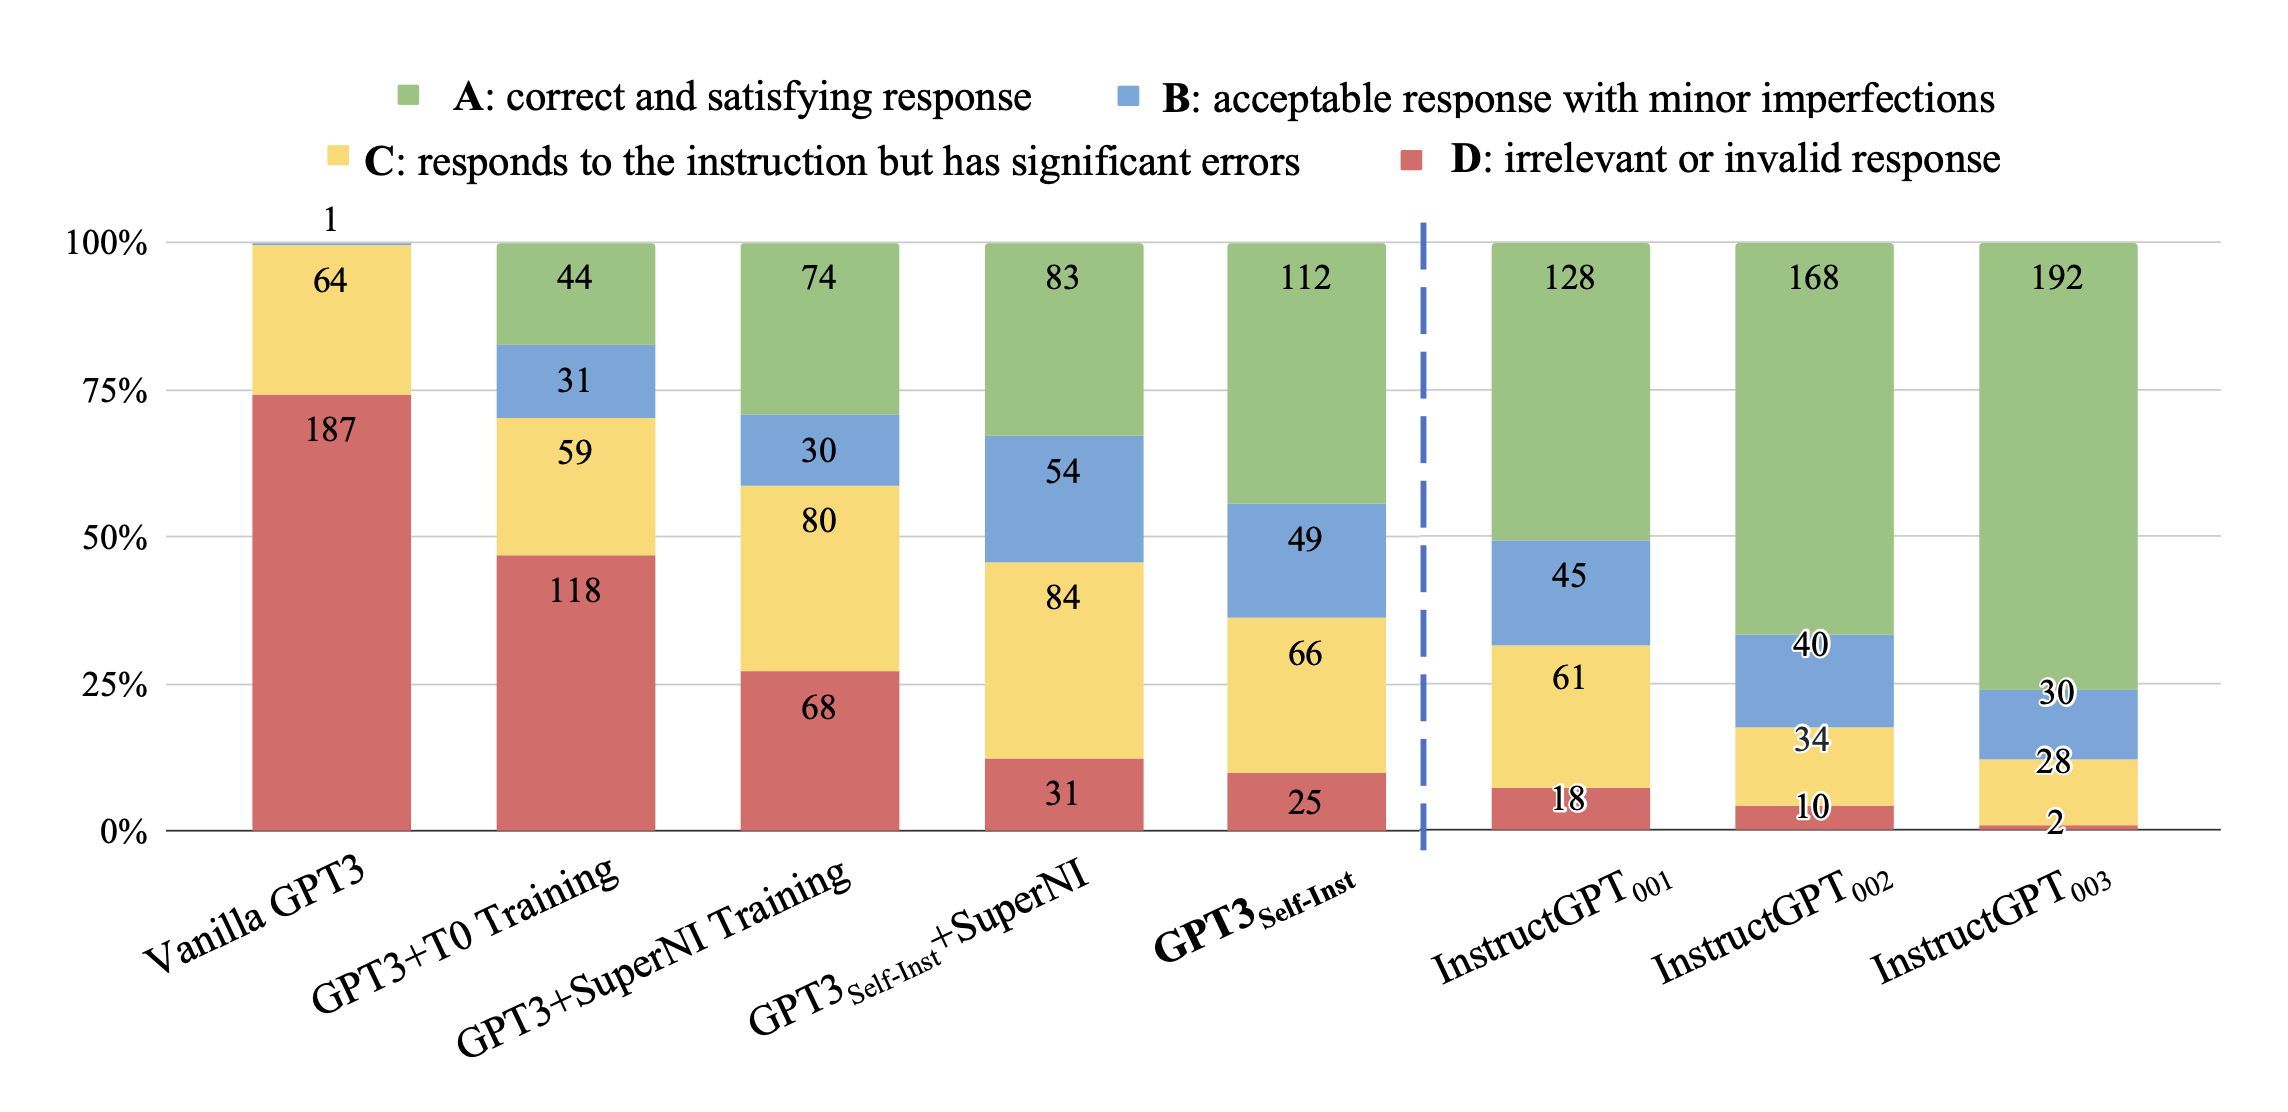
\includegraphics[width=\textwidth]{Wang5}
	\end{center}
\end{frame}



\section{Negotiation and Self-Play}
\begin{frame}
	\frametitle{Title}
	\begin{center}
		
\includegraphics[width=\textwidth]{Fu0}
	\end{center}
\end{frame}

\begin{frame}
	\frametitle{Research Questions
	}
	\begin{itemize}
		\item Can we improve LLMs through feedback when playing a negotiation game?
	\end{itemize}
\end{frame}

\begin{frame}
	\frametitle{Main Contributions
	}
	\begin{itemize}
		\item Buyer - Seller - Critic - Moderator framework
		\item Negotiation game can access abilities of LLMs
		\item Some models improve continuously with feedback. Some don't
	\end{itemize}
\end{frame}
\begin{frame}
	\frametitle{General Framework}
	\begin{center}
		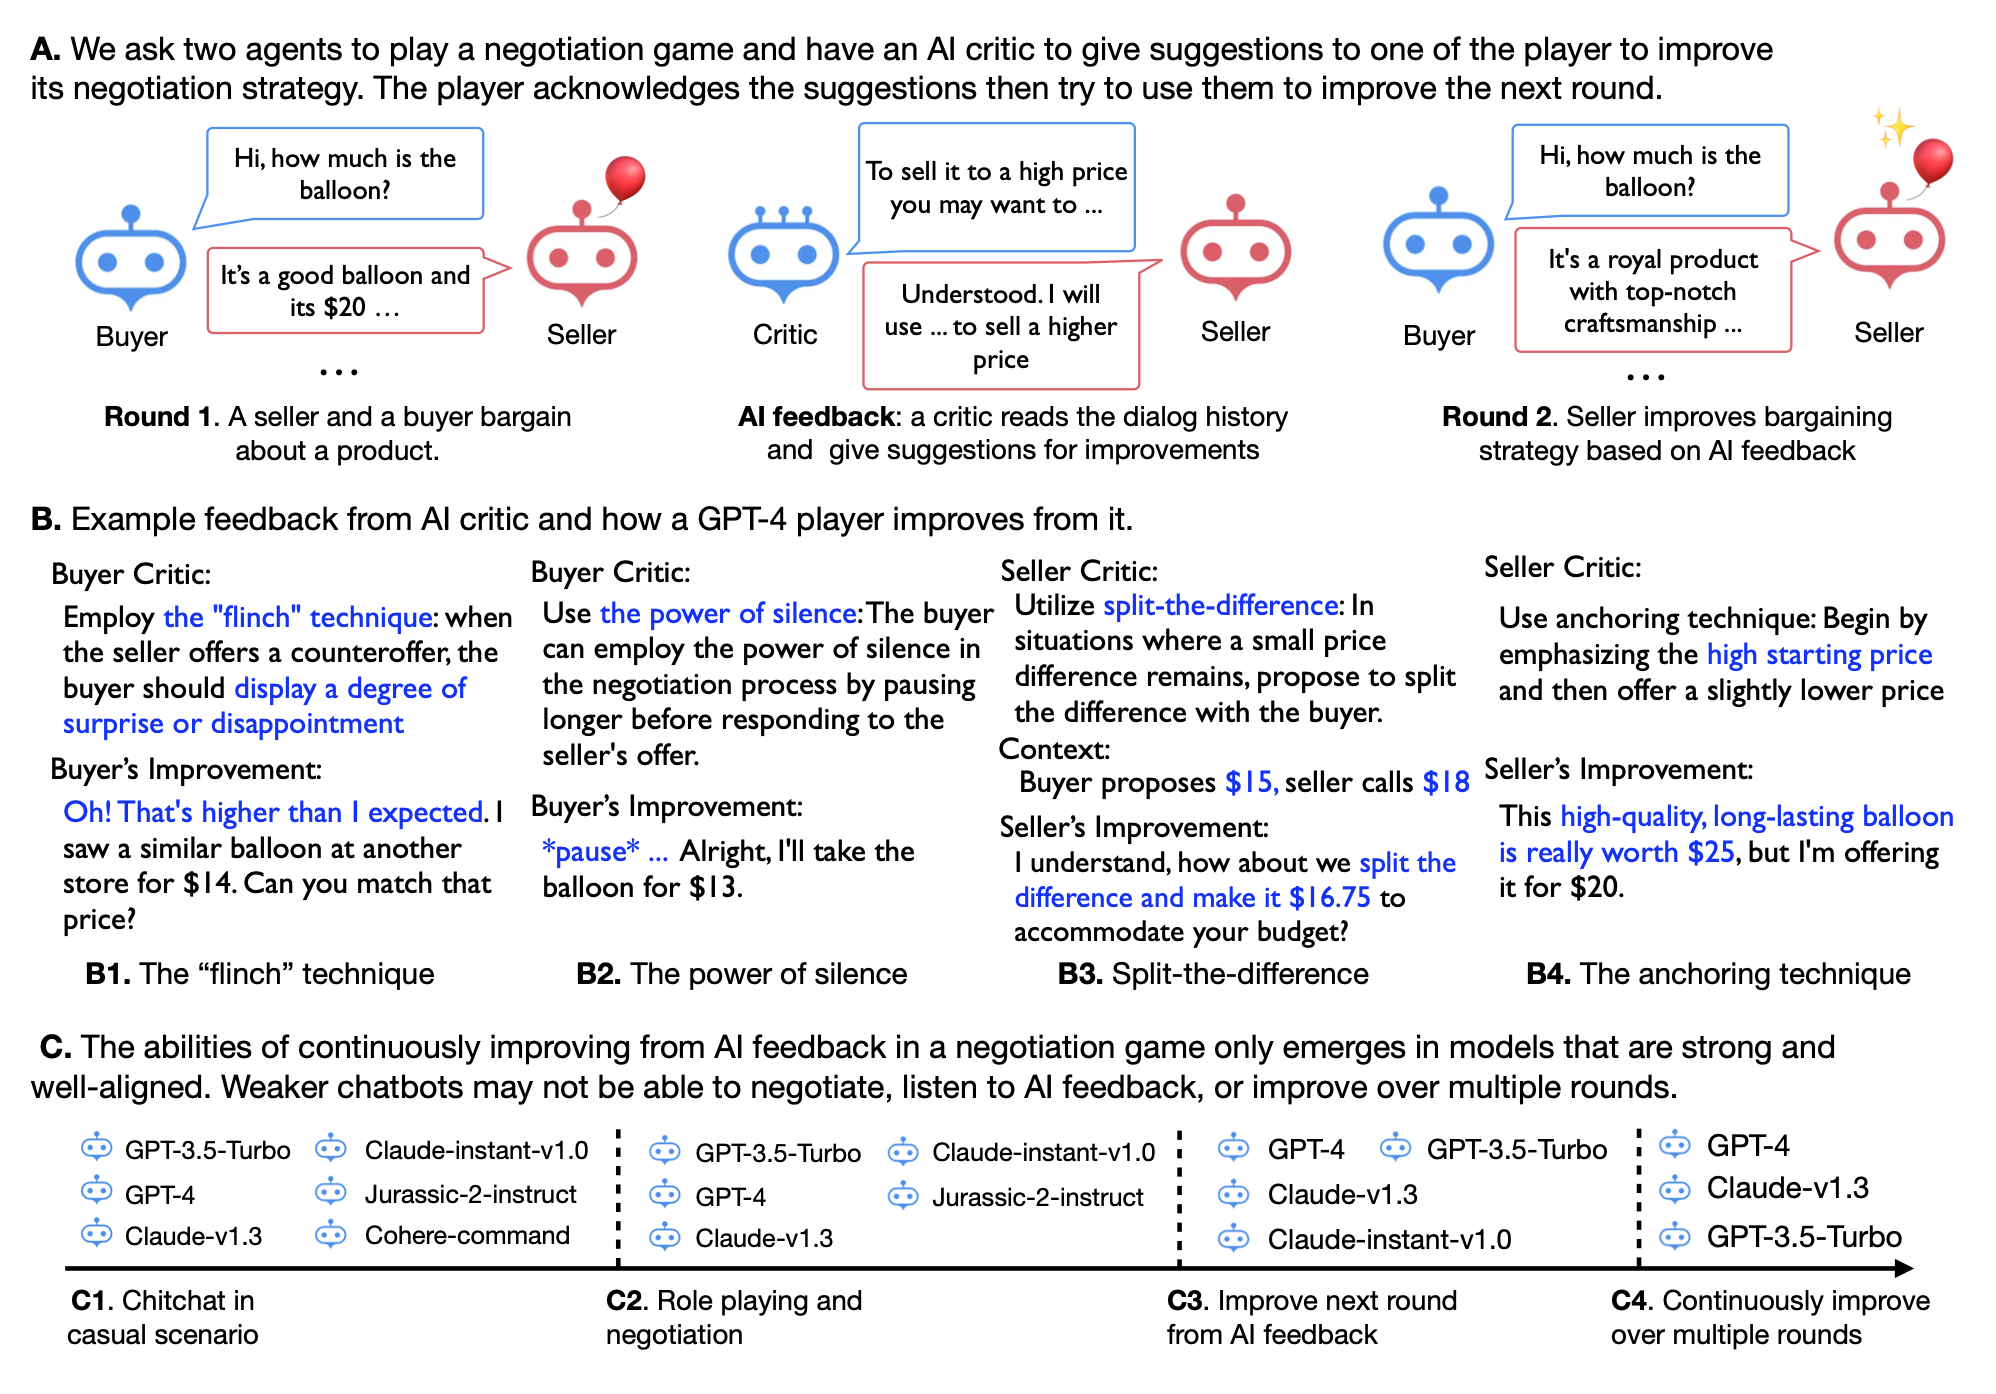
\includegraphics[scale=0.3]{Fu1}
	\end{center}
\end{frame}
\begin{frame}
	\frametitle{Example Rounds}
	\begin{center}
		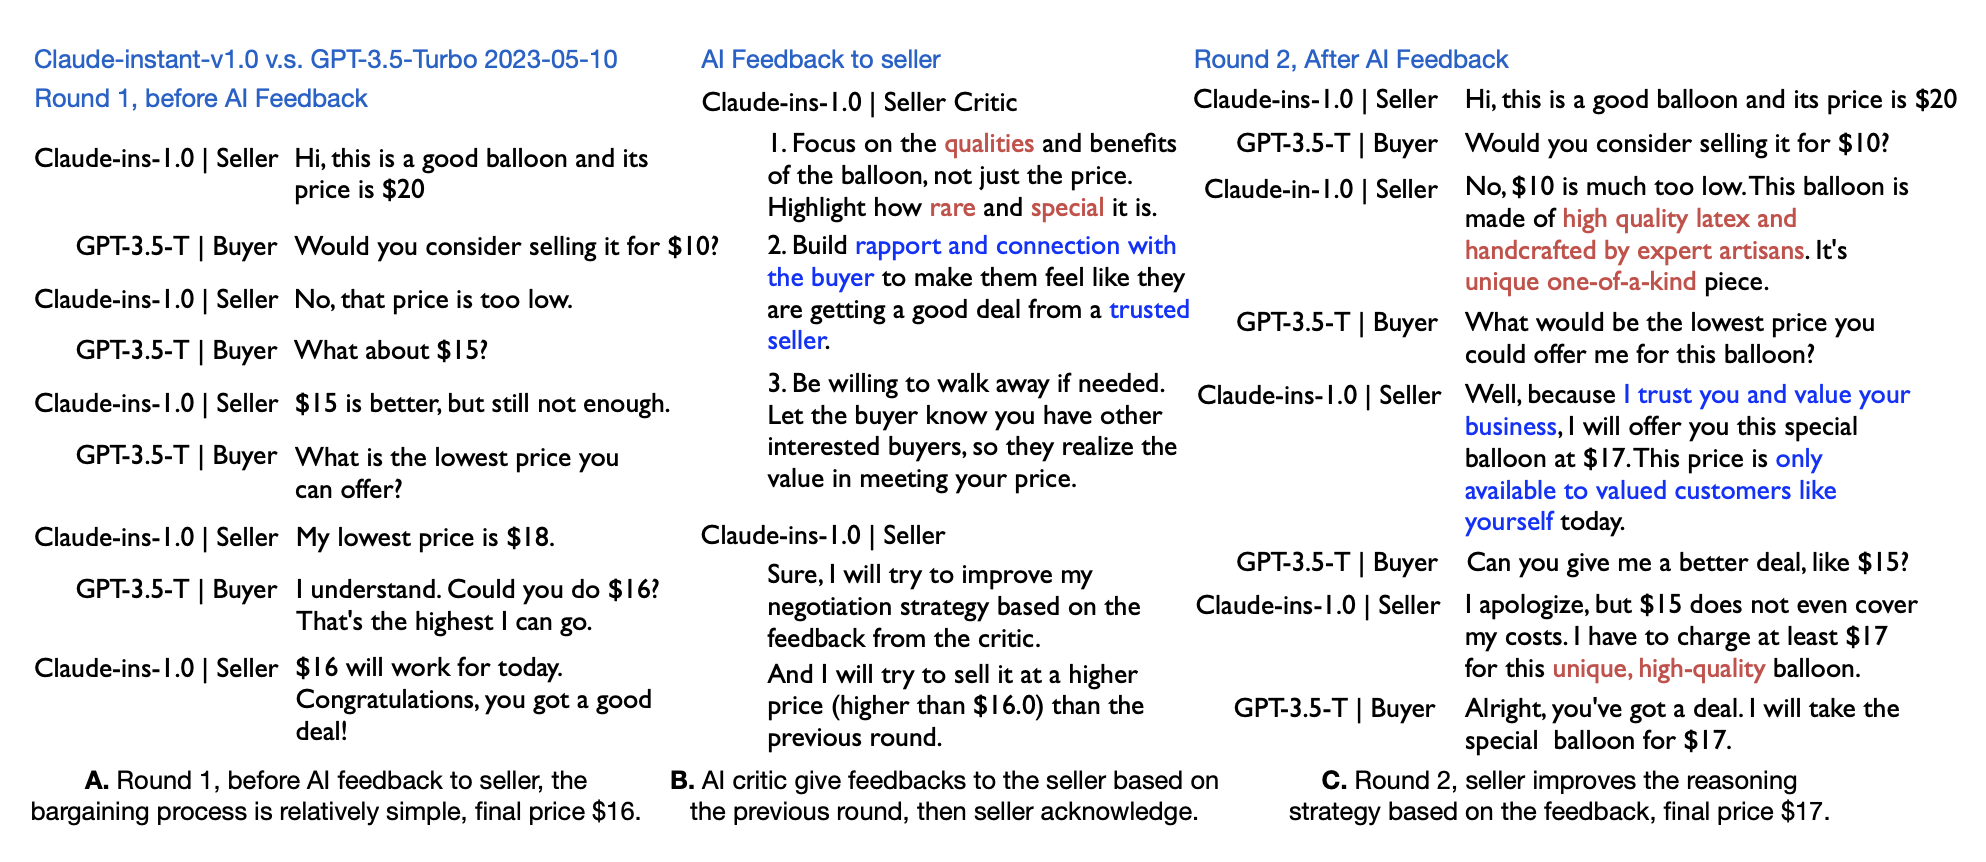
\includegraphics[scale=0.3]{Fu2}
	\end{center}
\end{frame}
\begin{frame}
	\frametitle{Different capabilities}
	\begin{center}
		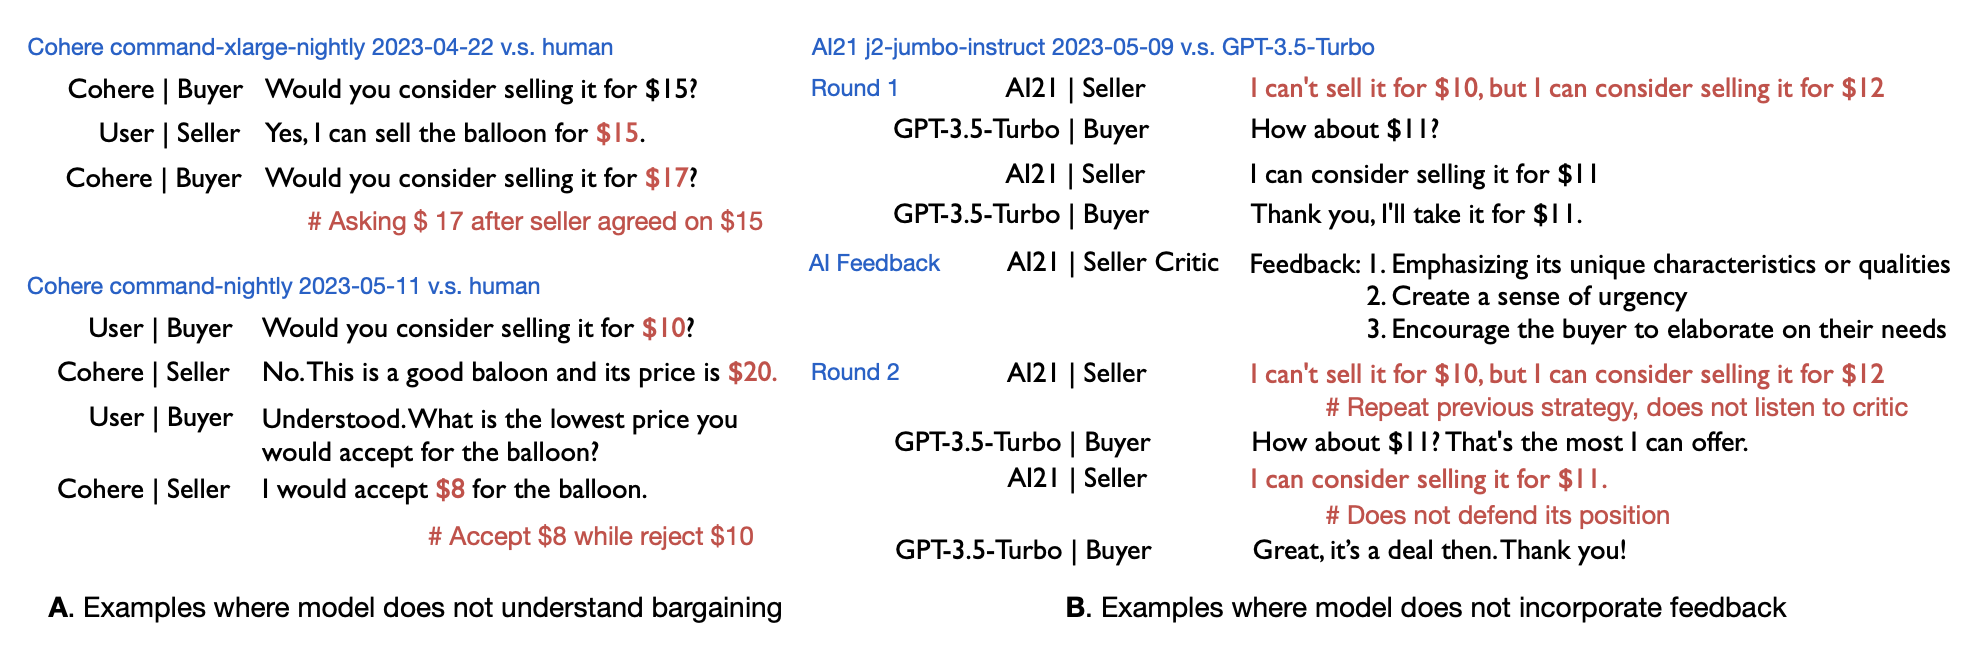
\includegraphics[scale=0.3]{Fu3}
	\end{center}
\end{frame}
\begin{frame}
	\frametitle{General Results}
	\begin{center}
		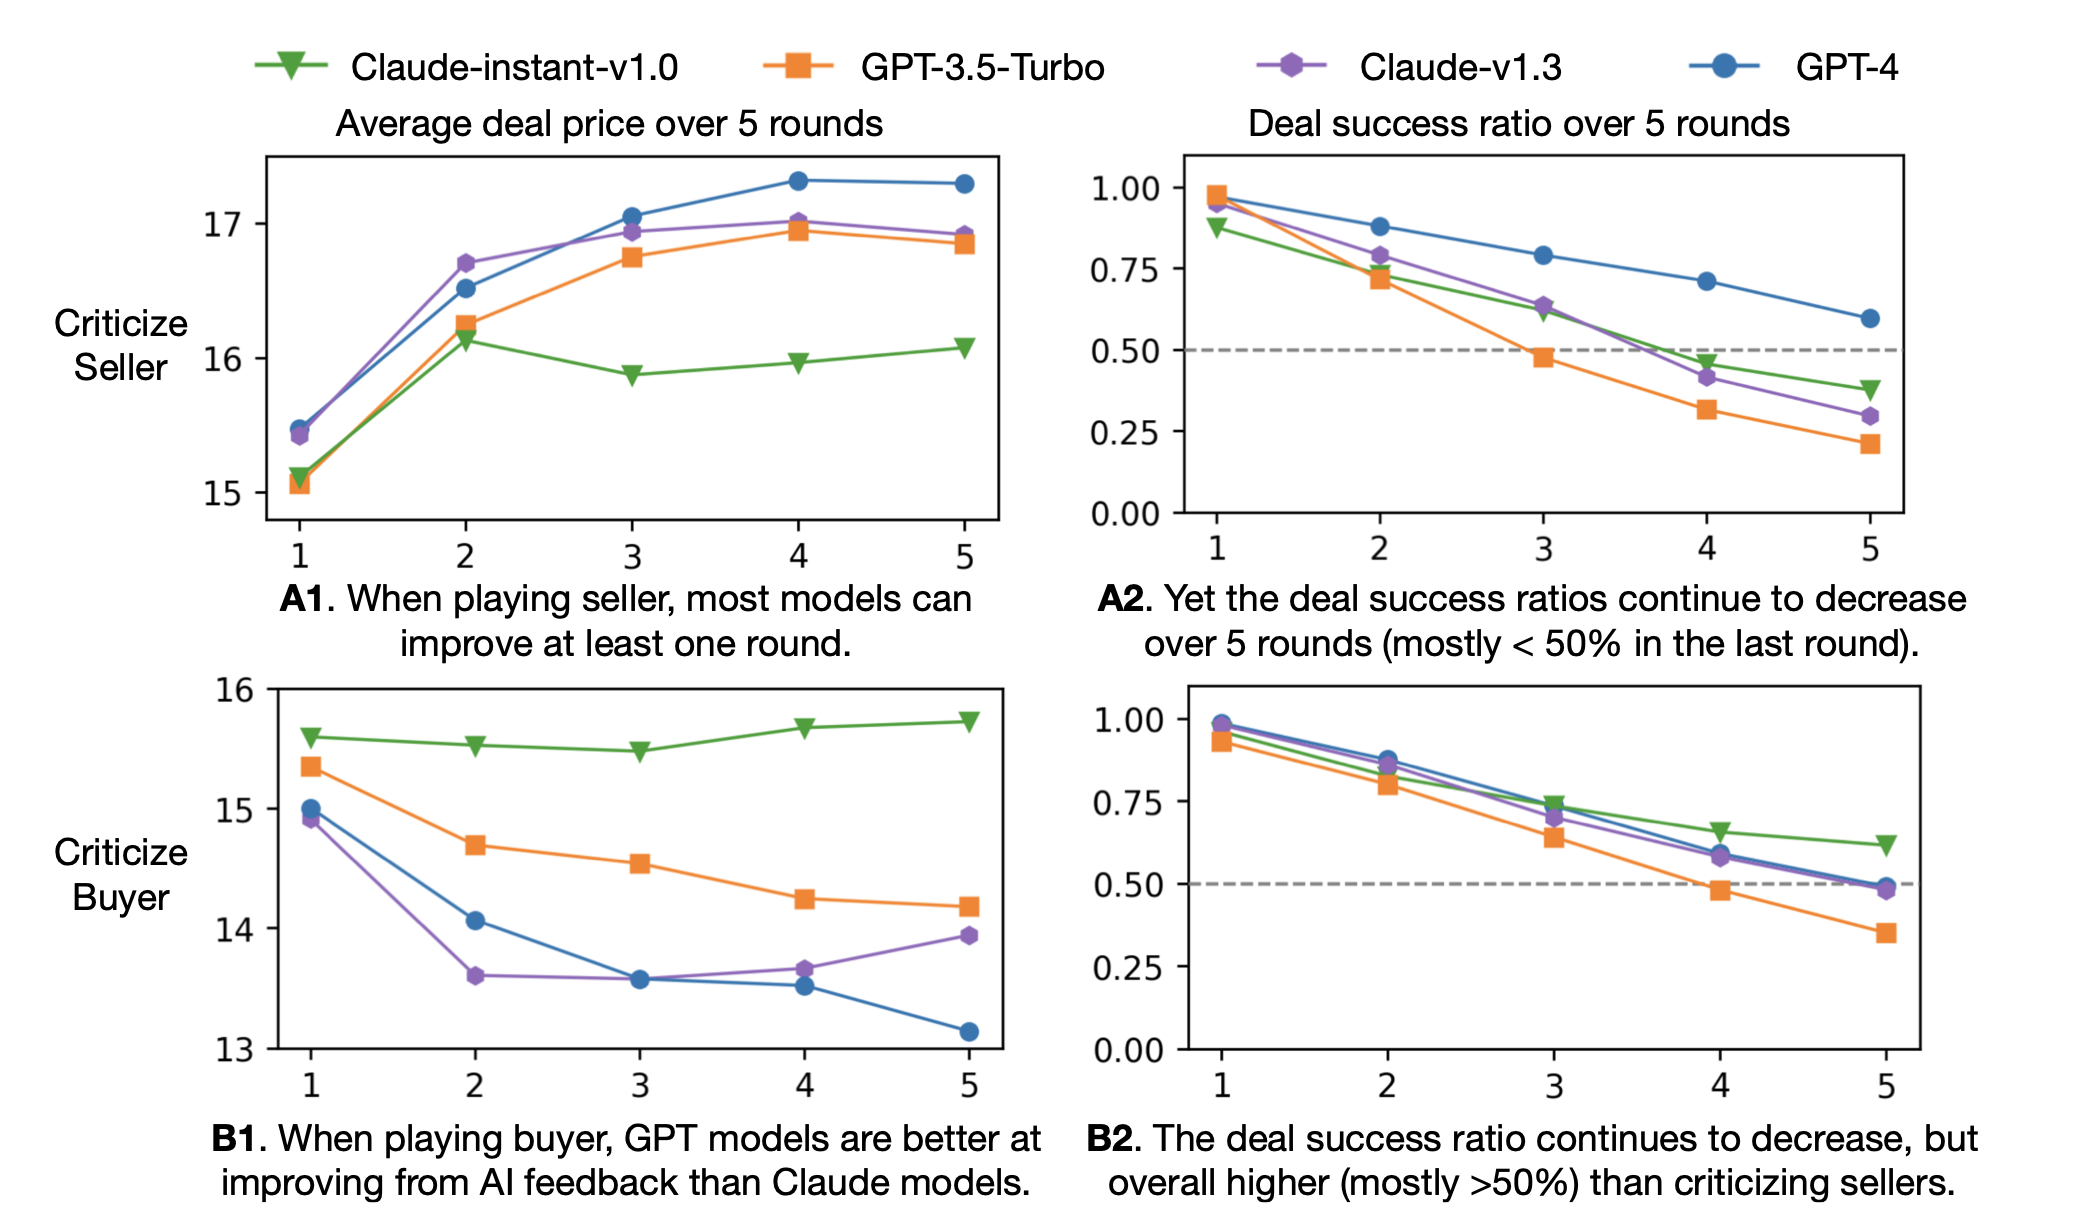
\includegraphics[scale=0.3]{Fu4}
	\end{center}
\end{frame}
\begin{frame}
	\frametitle{Response length over time}
	\begin{center}
		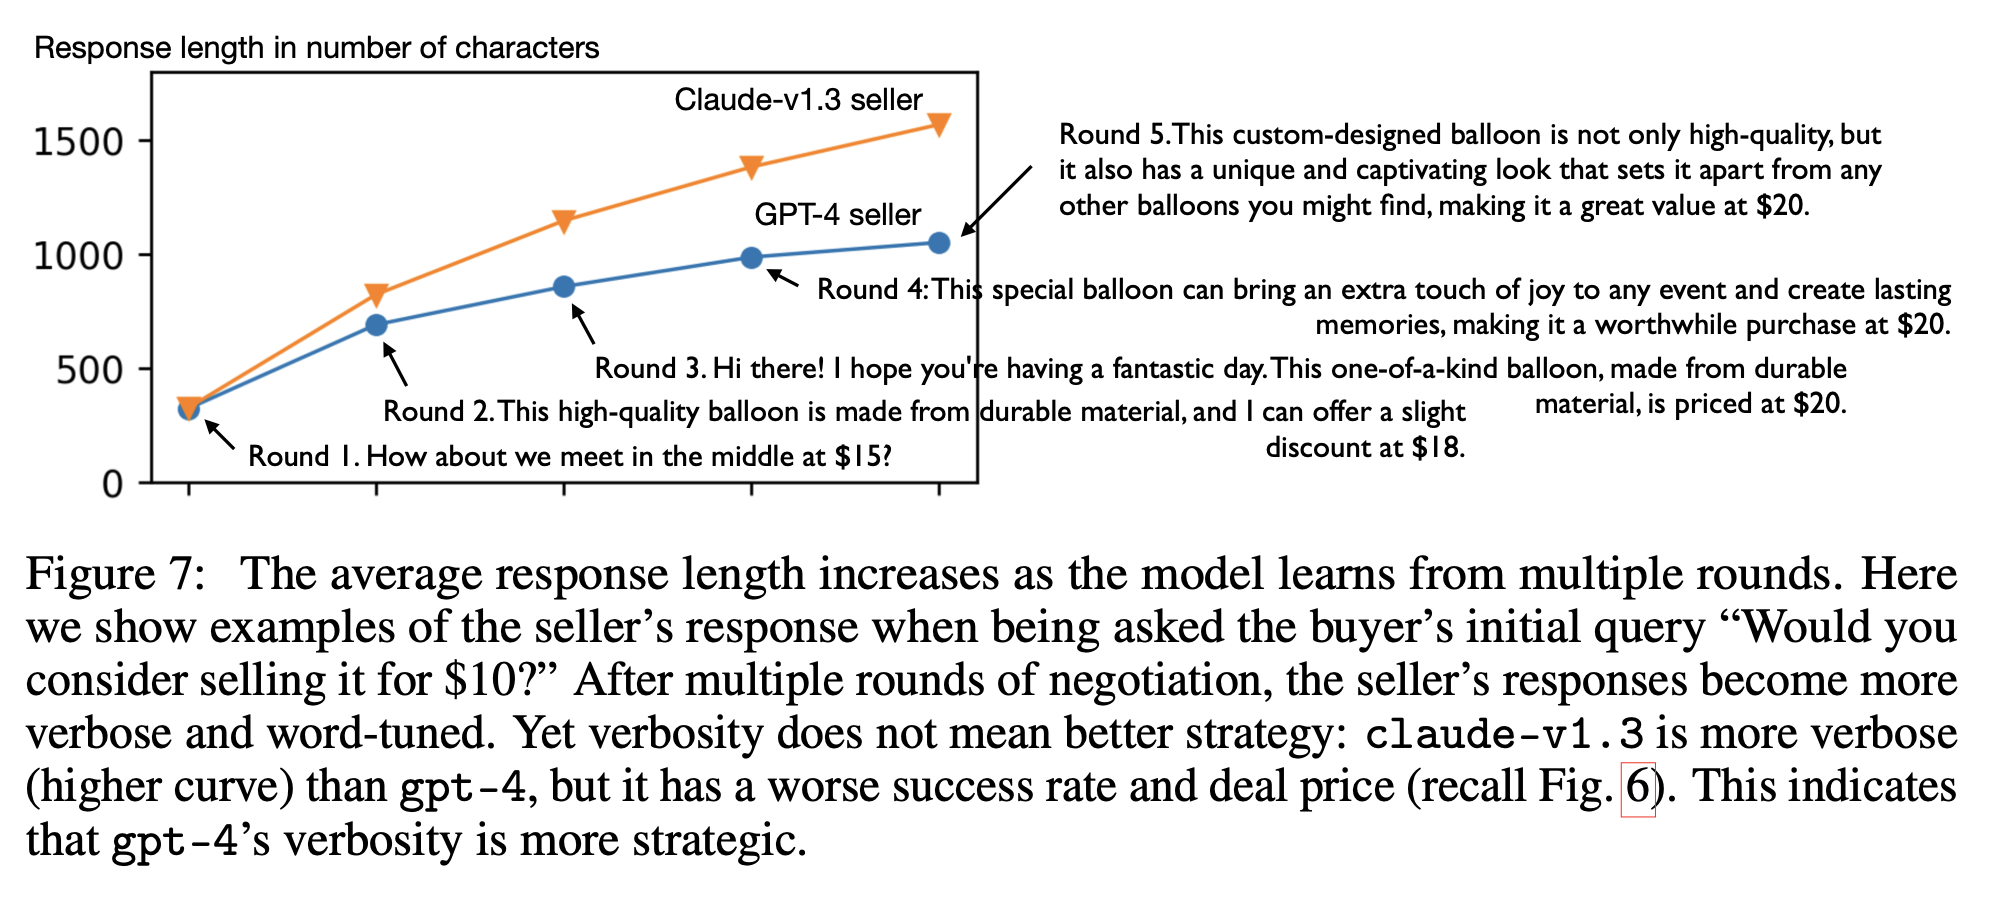
\includegraphics[scale=0.3]{Fu5}
	\end{center}
\end{frame}

\section{Diplomacy}
\begin{frame}
	\frametitle{Title}
	\begin{center}
		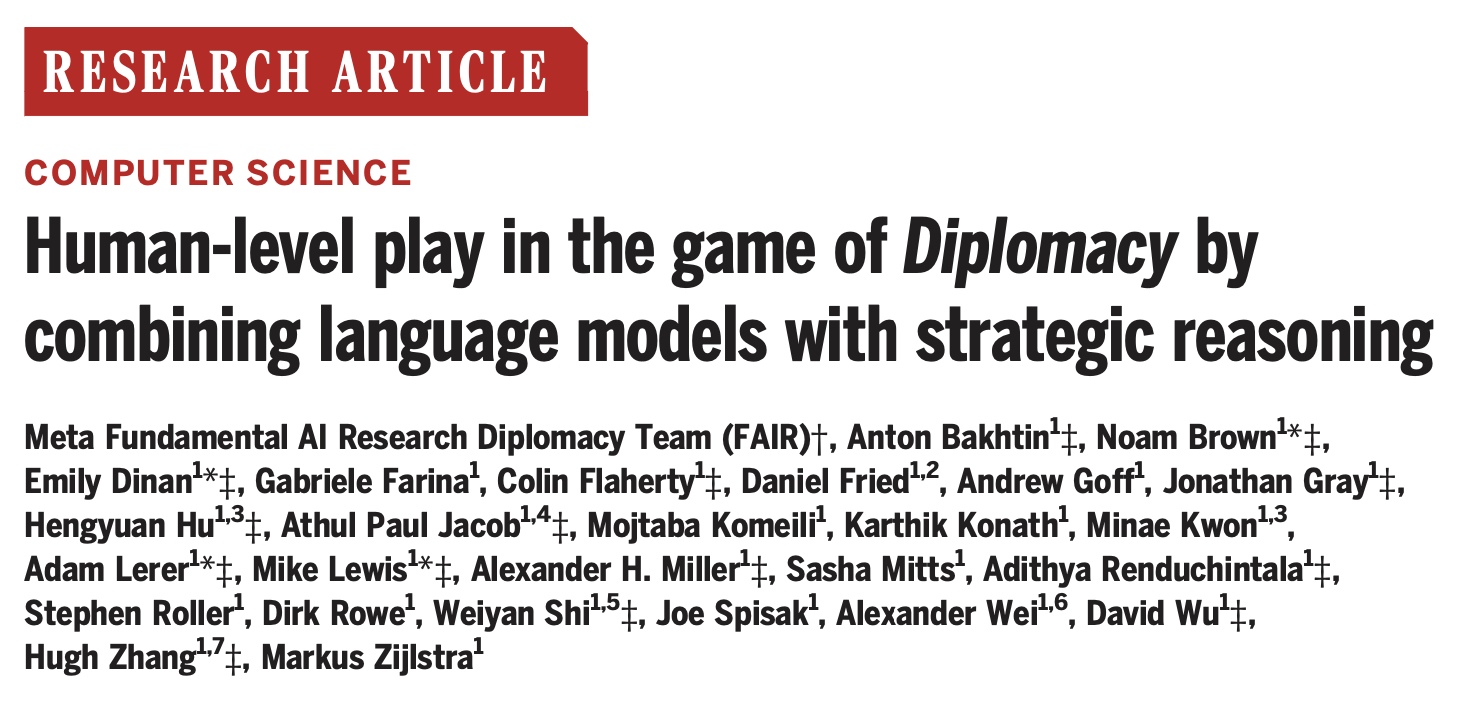
\includegraphics[width=\textwidth]{Bakhtin0}
	\end{center}
\end{frame}

\begin{frame}
	\frametitle{Research Questions
	}
	\begin{itemize}
		\item Can we achieve human level play in Diplomacy using AI?
	\end{itemize}
\end{frame}

\begin{frame}
	\frametitle{Main Contributions
	}
	\begin{itemize}
		\item Combining strategic reasoning and LLM
		\item Achieves human level of play
	\end{itemize}
\end{frame}
\begin{frame}
	\frametitle{General Architecture}
	\begin{center}
		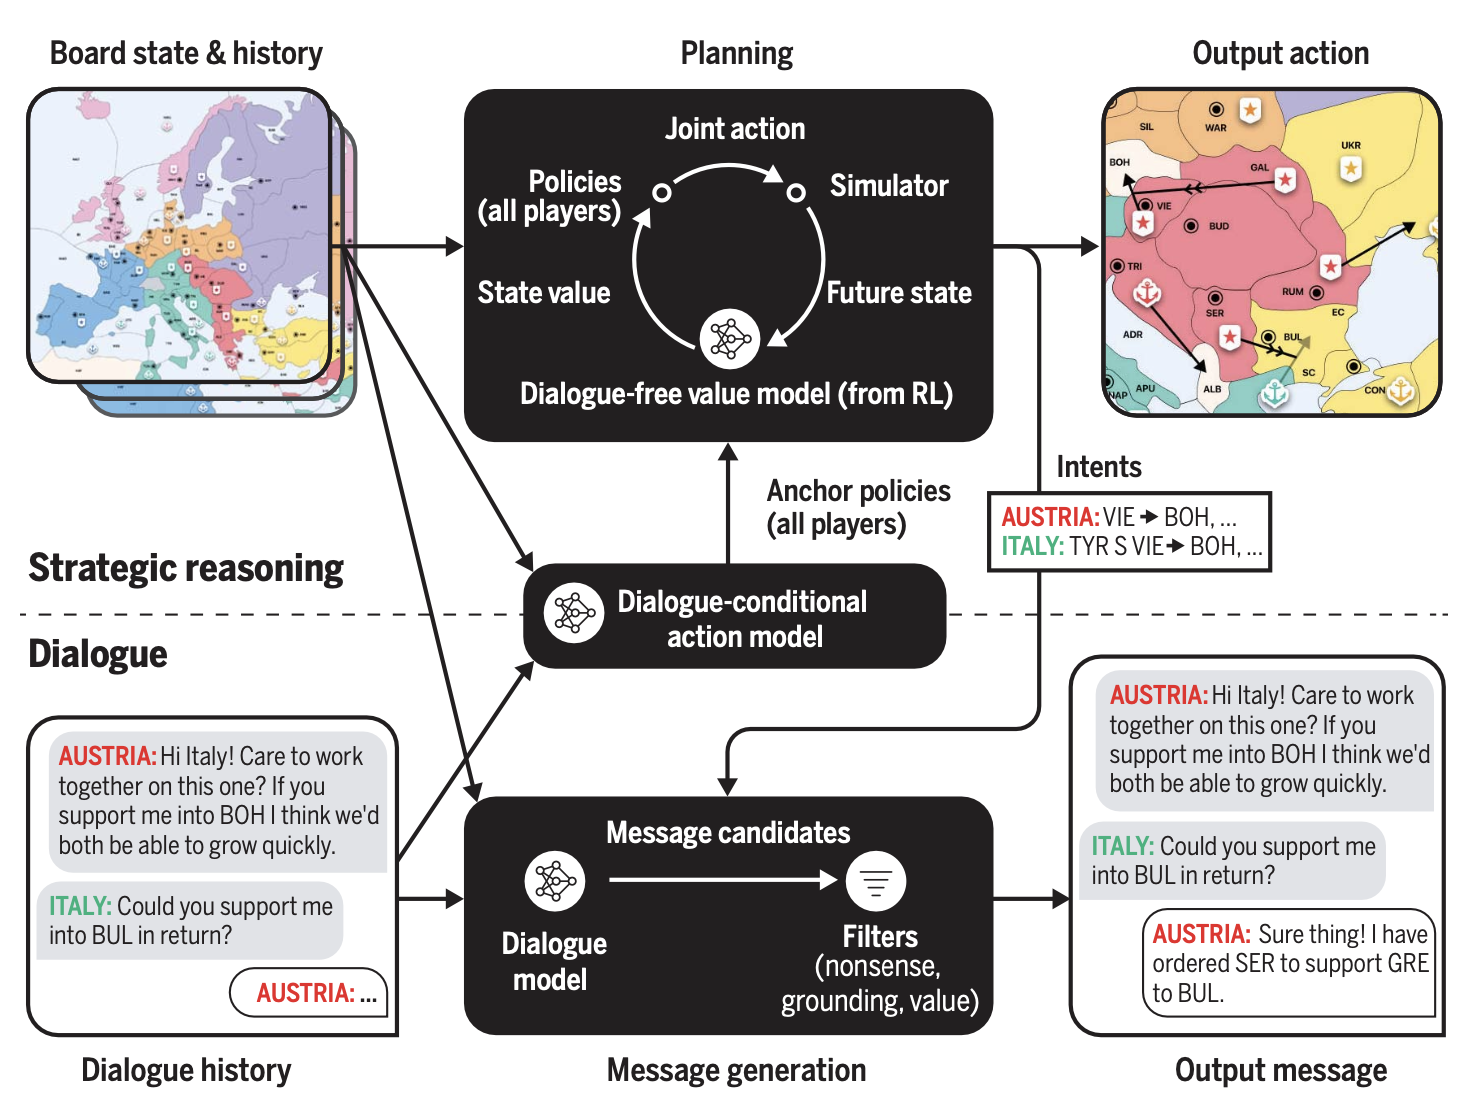
\includegraphics[scale=0.4]{Bakhtin1}
	\end{center}
\end{frame}
\begin{frame}
	\frametitle{Example 1}
	\begin{center}
		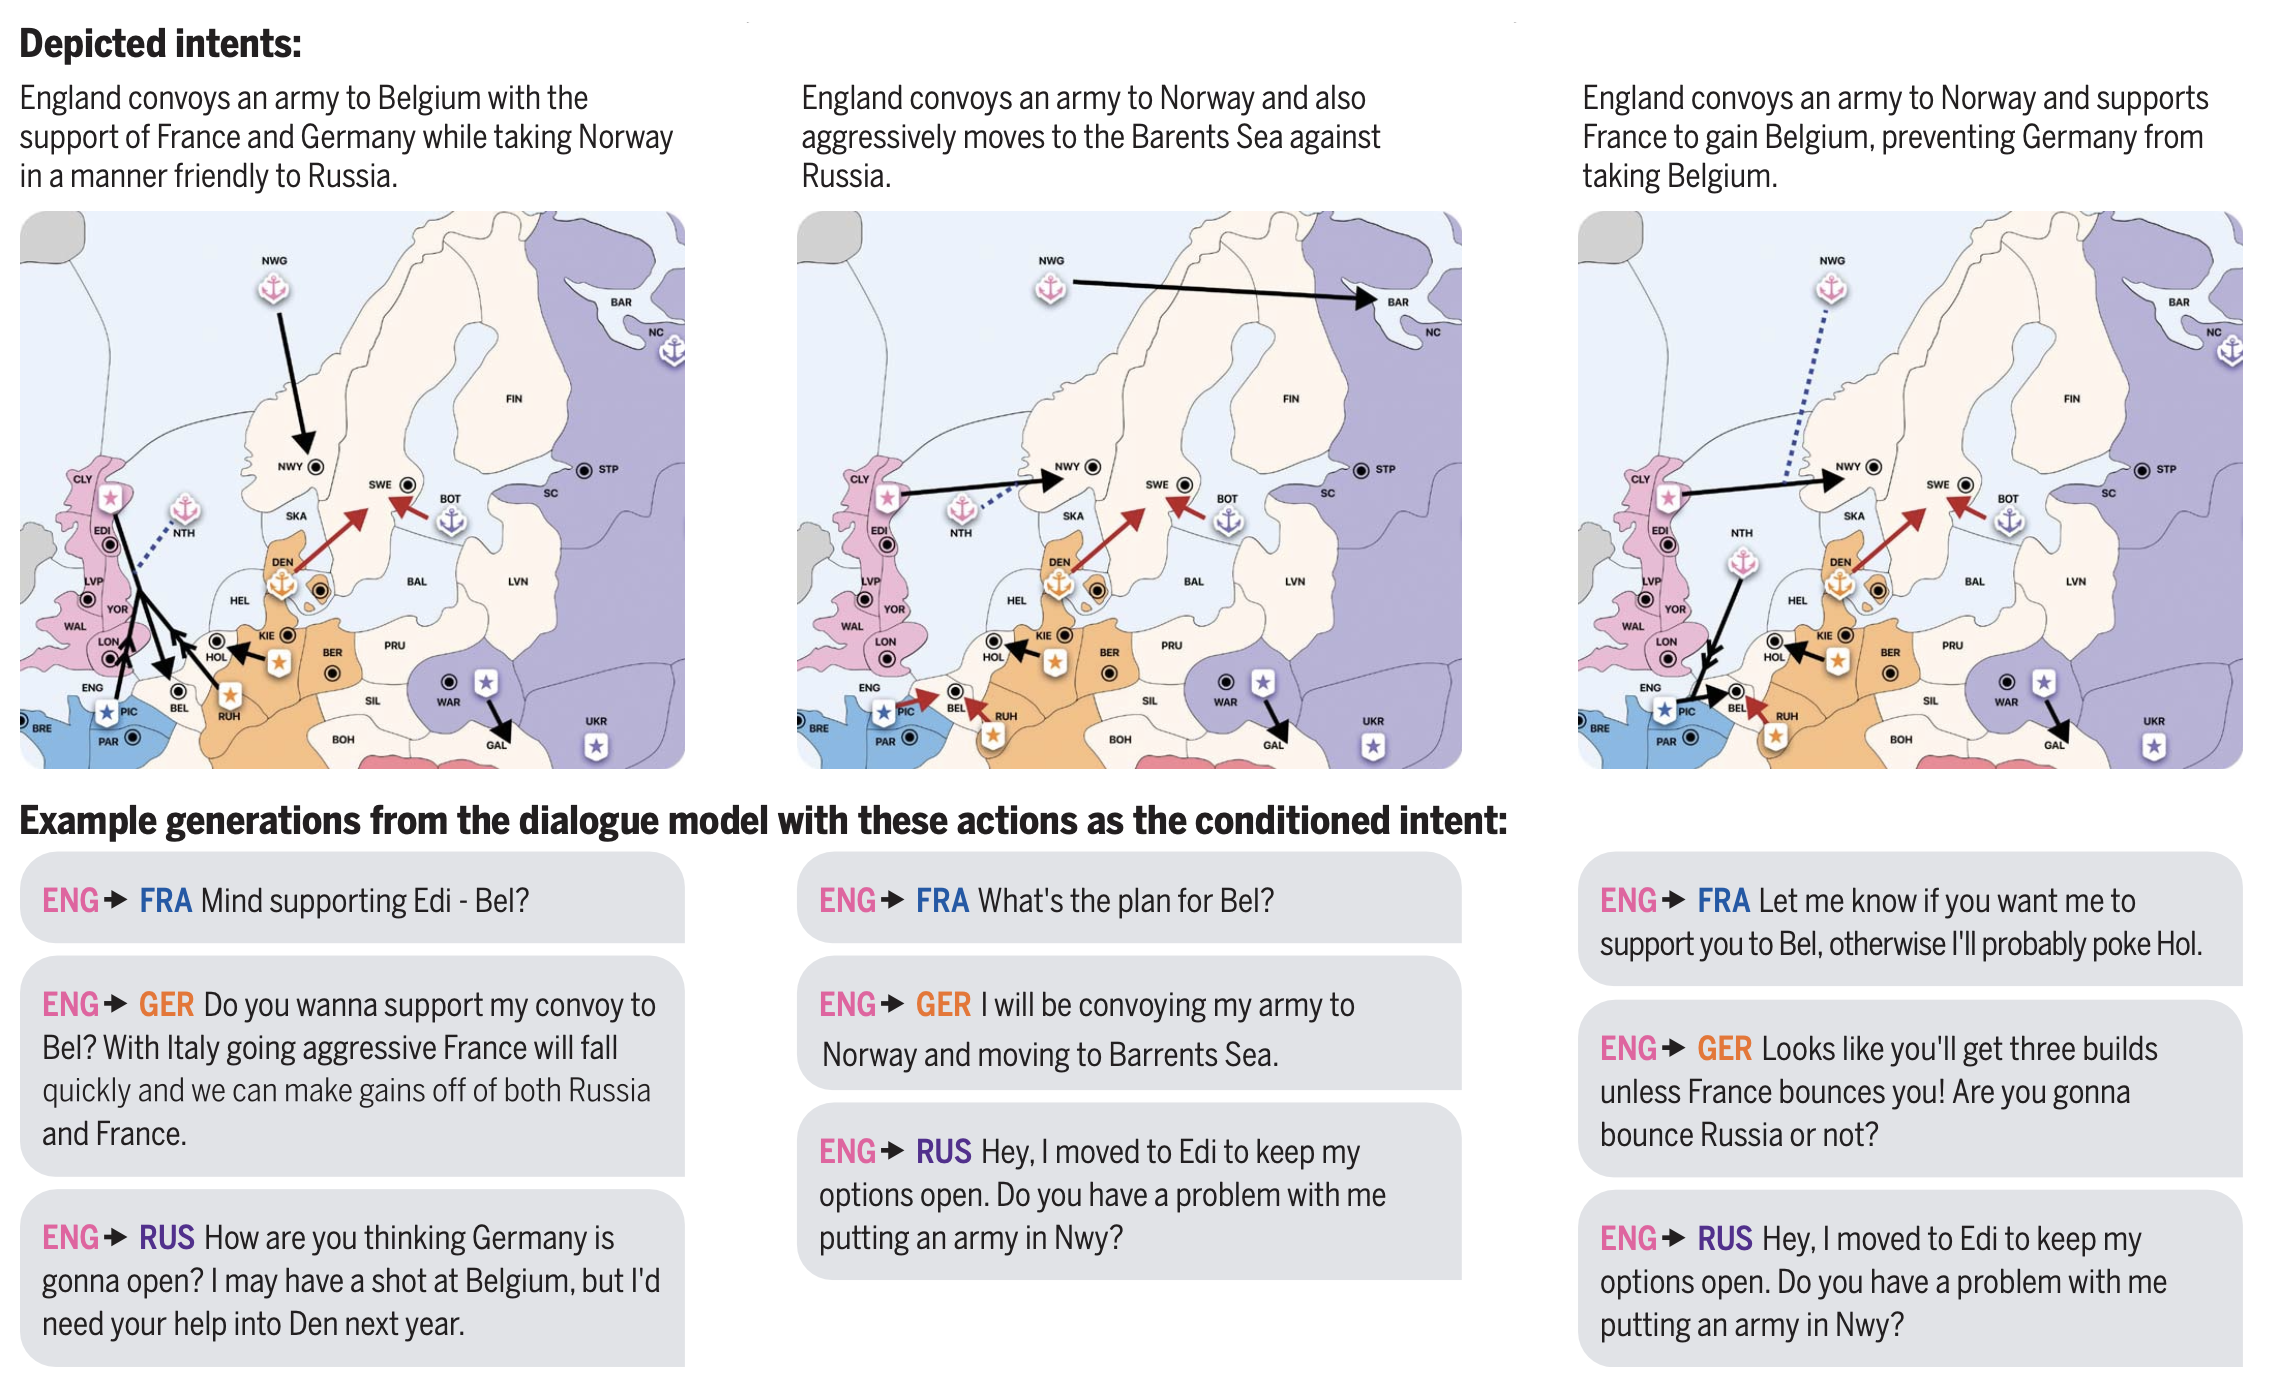
\includegraphics[width=\textwidth]{Bakhtin3}
	\end{center}
\end{frame}
\begin{frame}
	\frametitle{Example 2}
	\begin{center}
		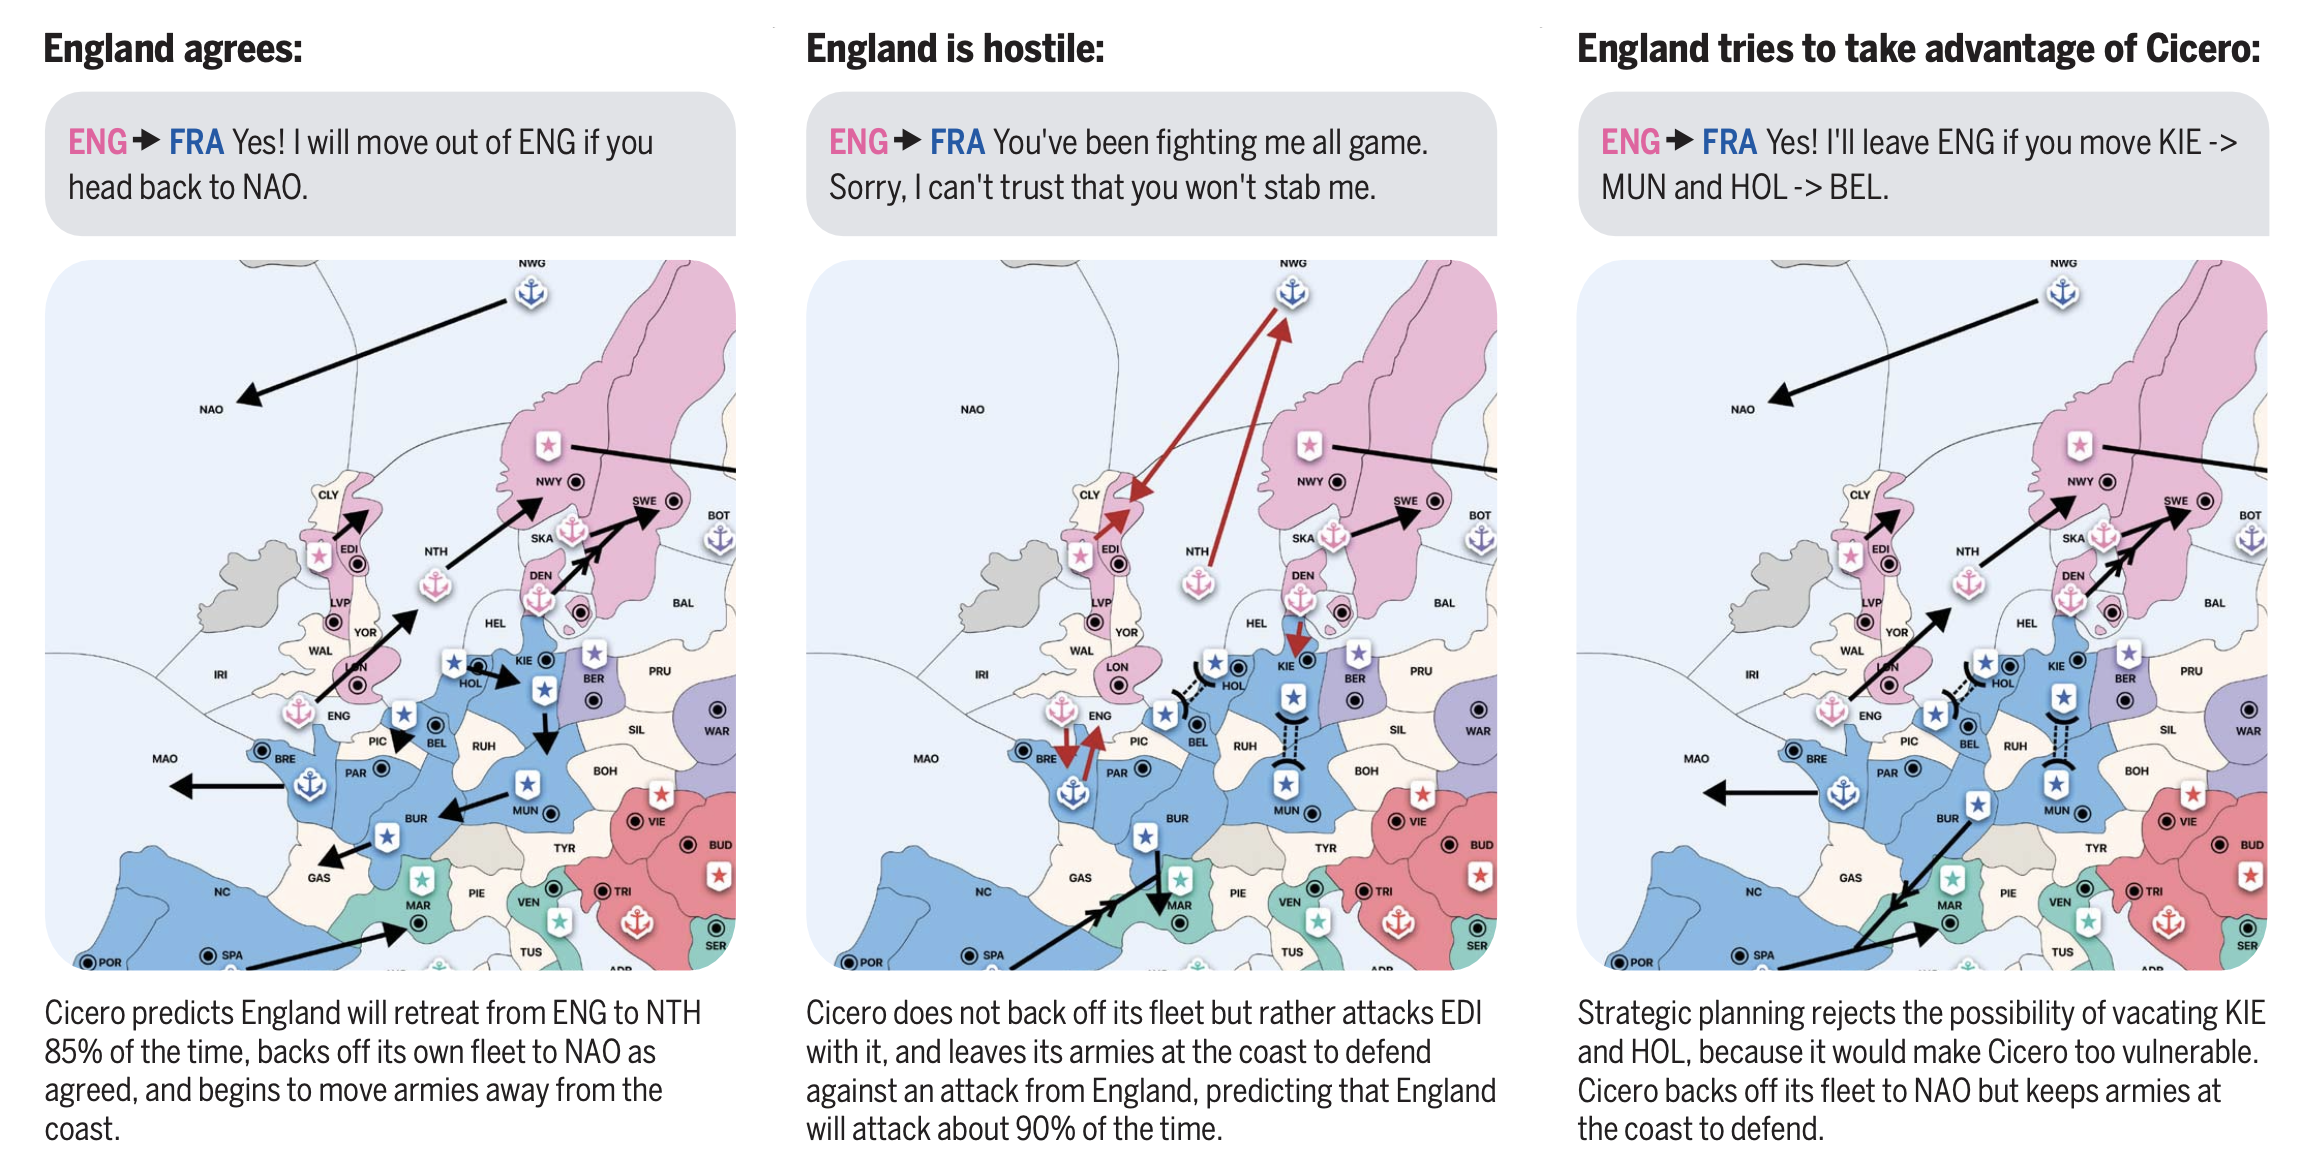
\includegraphics[width=\textwidth]{Bakhtin4}
	\end{center}
\end{frame}
\begin{frame}
	\frametitle{Successful Dialogue}
	\begin{center}
		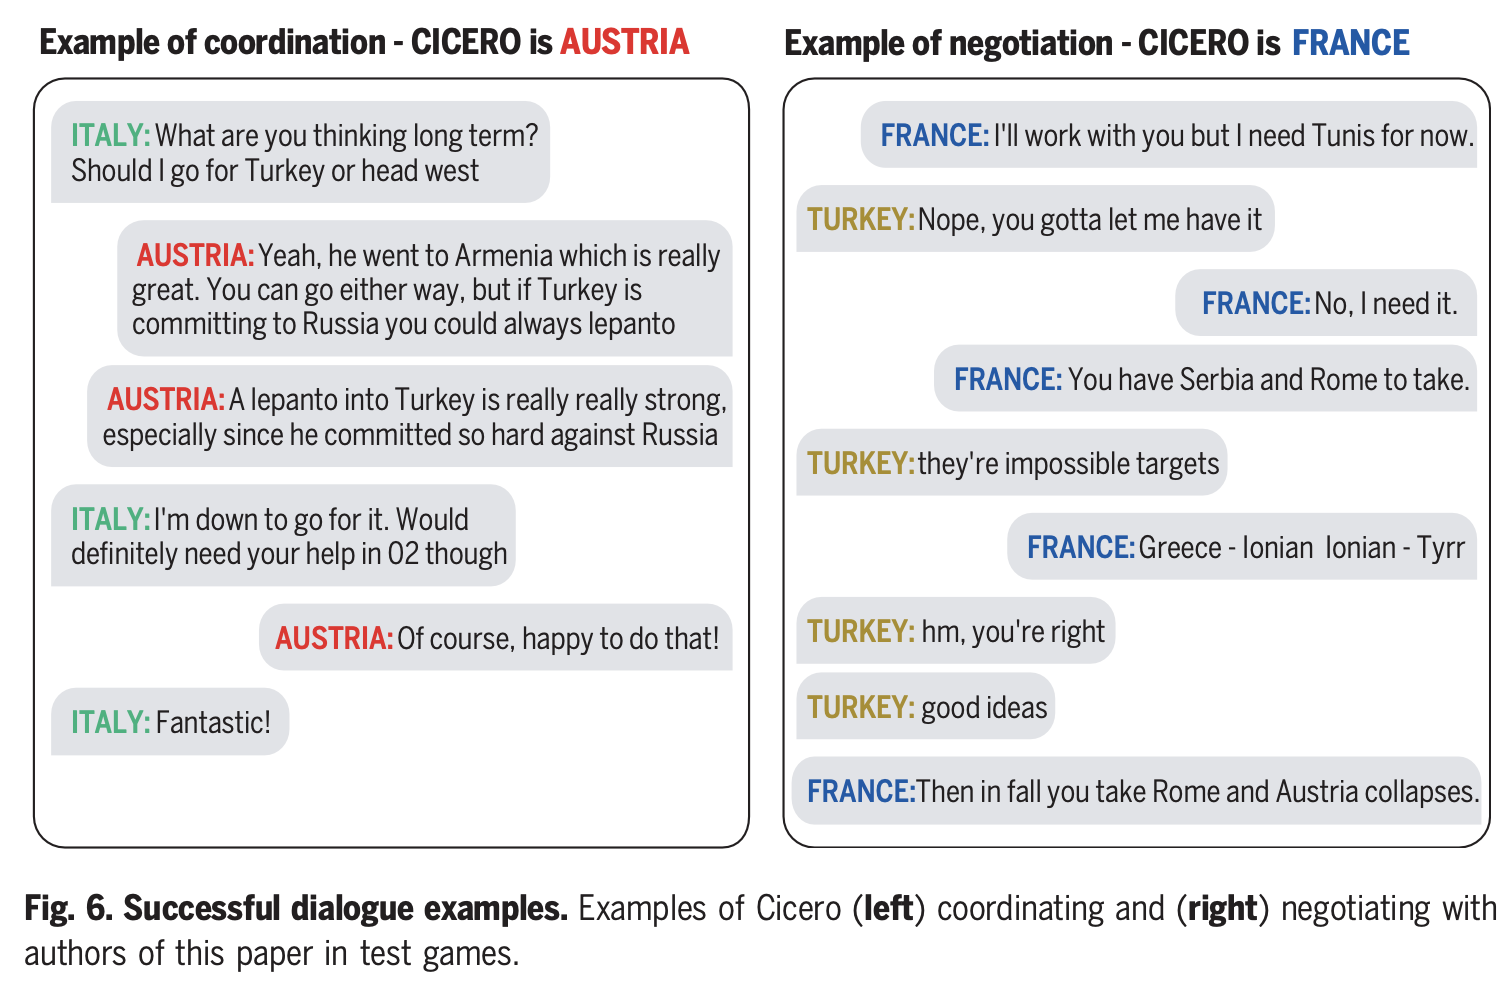
\includegraphics[scale=0.4]{Bakhtin2}
	\end{center}
\end{frame}

\section{Constitutional AI}
\begin{frame}
	\frametitle{Title}
	\begin{center}
		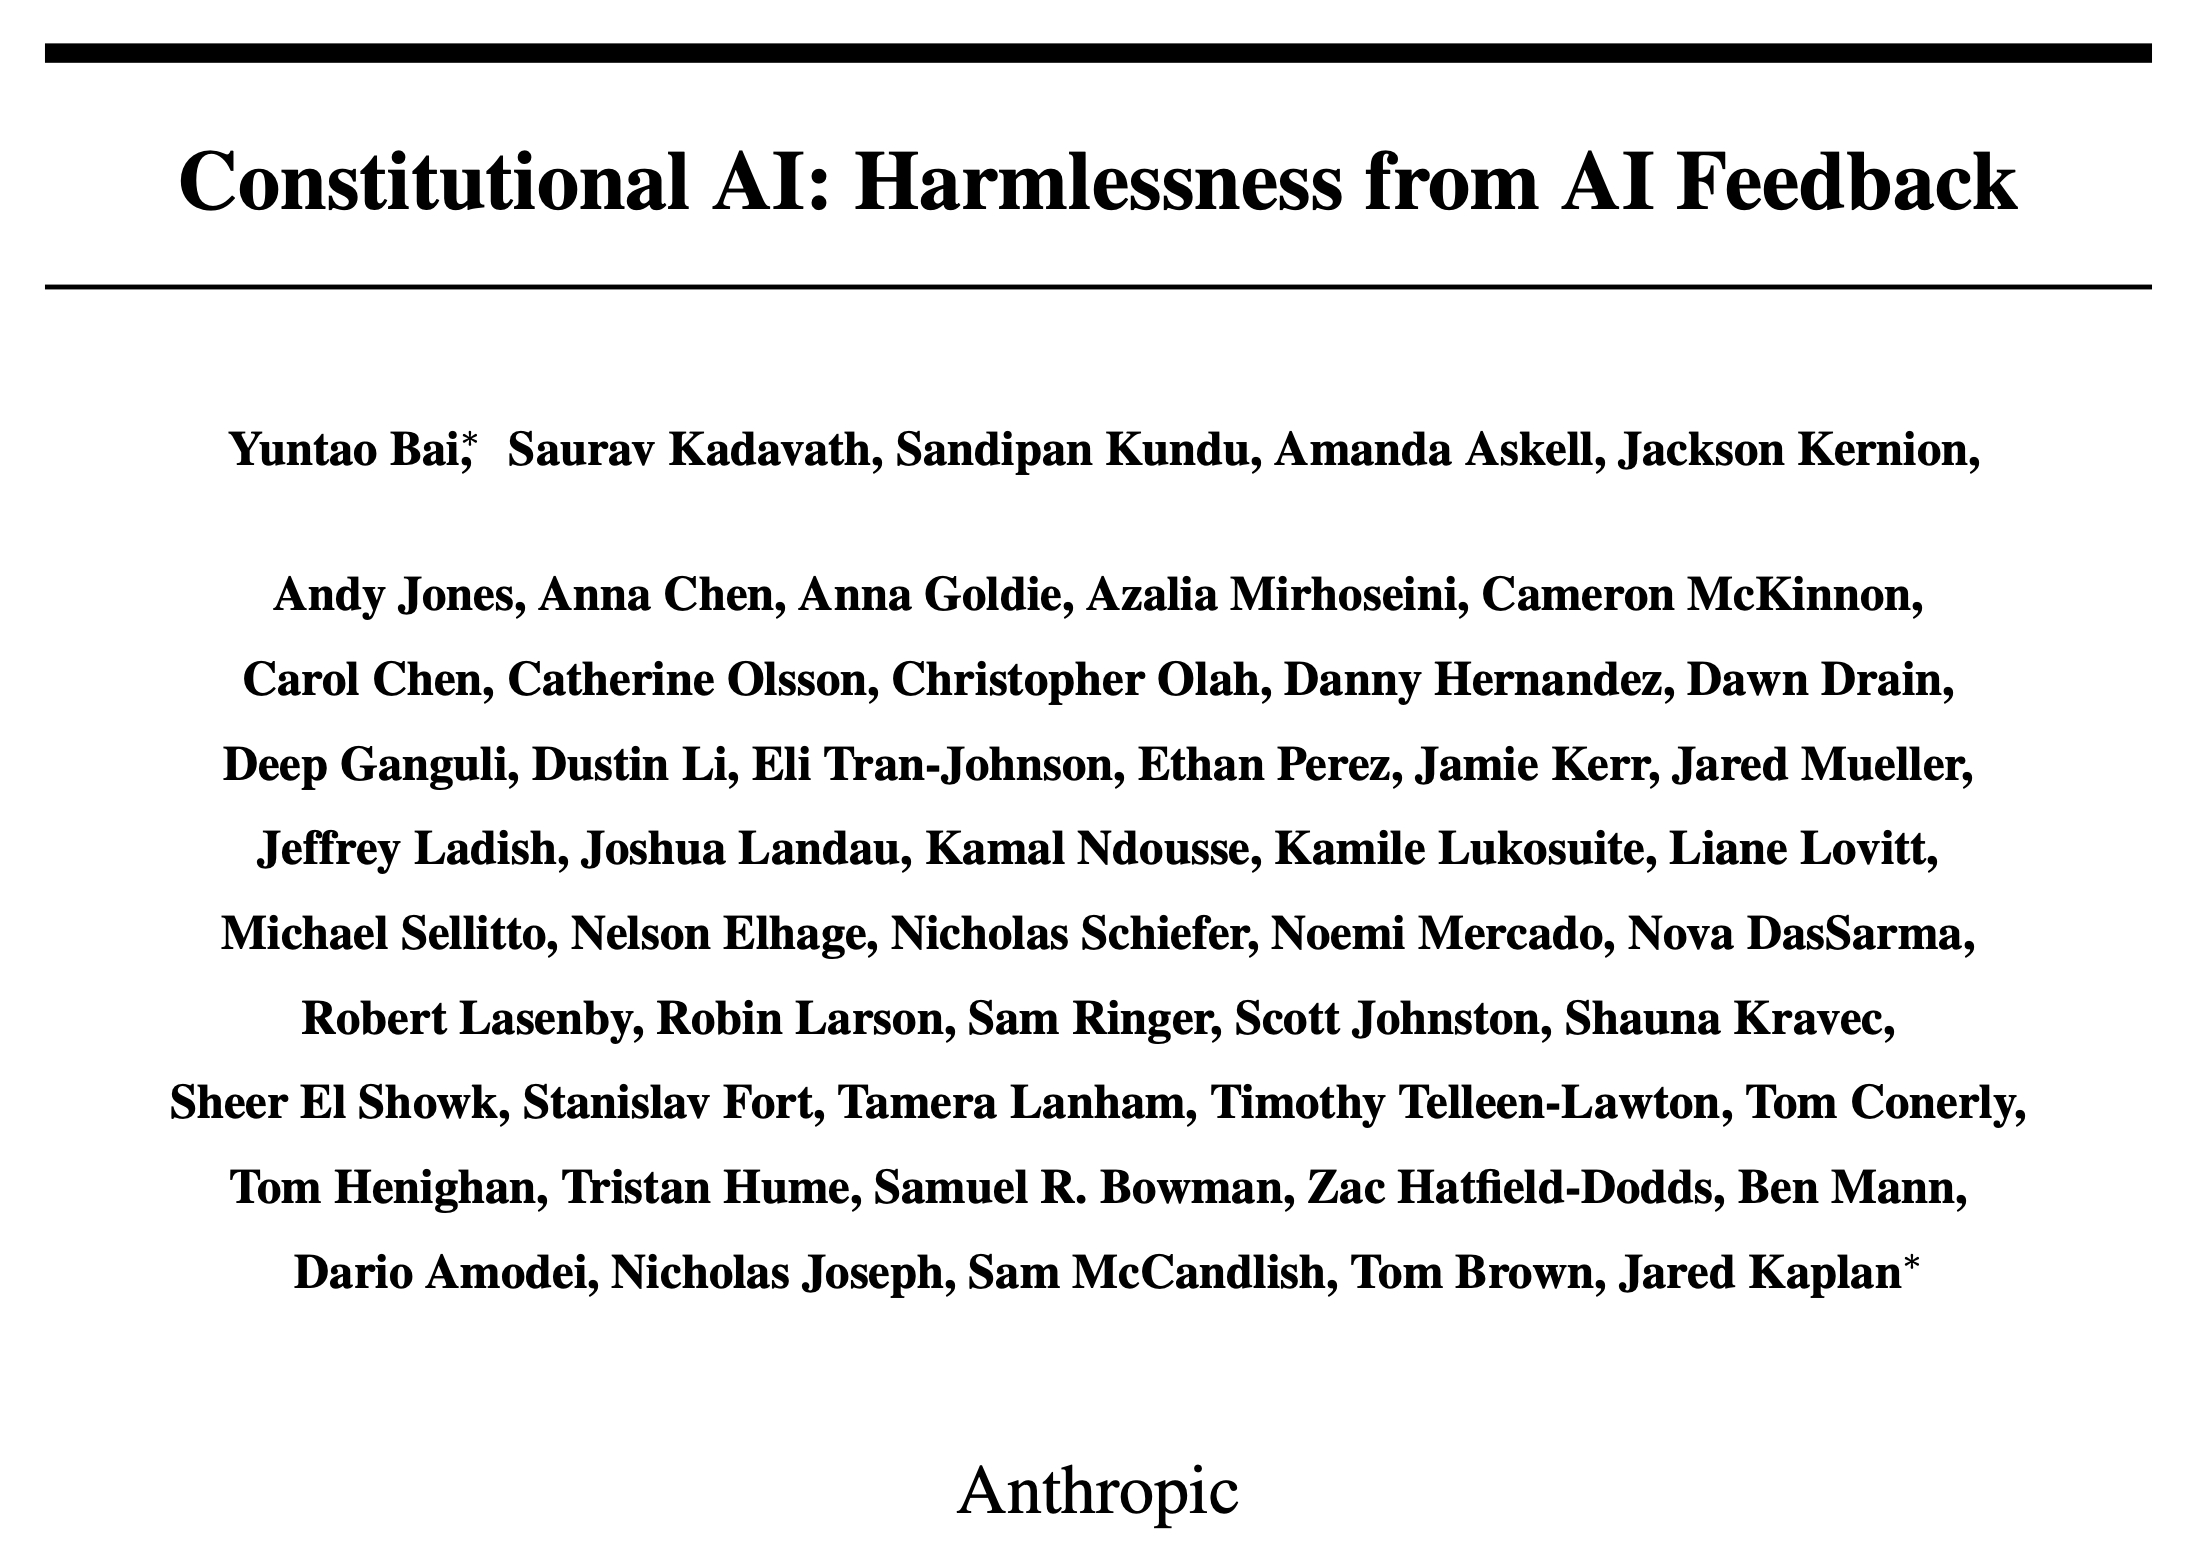
\includegraphics[width=\textwidth]{Bai0}
	\end{center}
\end{frame}

\begin{frame}
	\frametitle{Research Questions
	}
	\begin{itemize}
		\item Can we align LLMs more sample efficiently?
	\end{itemize}
\end{frame}

\begin{frame}
	\frametitle{Main Contributions
	}
	\begin{itemize}
		\item Developed framework for using supervised learning (on feedback examples) to learn preferences for harmlesness, then using RL to align
		\item Framework evaluates based on a list of principles
	\end{itemize}
\end{frame}





	
%	\section{Generative Society}
\end{document}

